\documentclass{mammoth}

\addbibresource{references.bib}

\begin{document}

\frontmatter

\begin{titlepage}

    \begin{center}
        \Large\scshape
        School of Electrical Engineering,\\Computing and Mathematical Sciences
    \end{center}

    \vfill
    \vspace{3\baselineskip}

    \begin{center}
        \Huge\bfseries
        Bayesian Hierarchical Modelling of Equipment Reliability in Mining: A Pragmatic Approach
    \end{center}

    \vfill
    \vspace{3\baselineskip}

    \begin{center}
        \huge\bfseries
        Ryan K. Leadbetter

        \Large\normalfont
        0000-0002-1942-3121
    \end{center}

    \vfill
    \vspace{3\baselineskip}

    \begin{center}
        \large
        Centre for Transforming Maintenance Through Data Science
    \end{center}

    \vfill

    \begin{center}
        \large\itshape
        This thesis is presented for the\\
        Degree of Doctor of Philosophy of\\
        Curtin University
    \end{center}

    \vfill

    \begin{center}
        \Large
        \textsc{February 2025}
    \end{center}

    \cleardoublepage
\end{titlepage}


\vspace*{2cm}

\noindent
\titlesc{Declaration}

\vfill
\vspace{3\baselineskip}

\noindent
To the best of my knowledge and belief this thesis contains no material previously published by any other person except where due acknowledgement has been made.

\vspace{14pt}

\noindent
This thesis contains no material which has been accepted for the award of any other degree or diploma in any university.

\vfill
\vspace{5cm}

\noindent
\begin{tabular}{@{}ll}
    Signature: & \hrulefill                \\
               & Ryan Leadbetter \hspace{5em} \\
               &                           \\
    Date:      & February 11, 2025             \\
\end{tabular}

\vspace*{3.5cm}

\clearpage

%%
%% This is a file demonstrating the use of the abstract file in the Curtin thesis skeleton
%% file. And can be used as infrastructure to build your thesis.
%%

\chapter*{Abstract} \addcontentsline{toc}{chapter}{Abstract}

From pit to port, the consistent and efficient operation of iron ore machinery is essential for maximizing profits. To this end, reliability modelling is an invaluable tool for improving the design and execution of the maintenance strategies that ensure the reliable operation of mining machinery. There are well established reliability models in the literature, but there is a discrepancy between this literature and what is actually done by practitioners in the mining industry; a theory-practice gap. This gap exists because of the imperfect reality of collecting data in the field--data sets that are small, incomplete, noisy, or all three--and the lack of methods for expanding reliability modelling to account for these imperfections. My industry-linked PhD has aimed to reduce this gap by demonstrating how Bayesian statistical modelling framework can address some of the common problems faced when fitting models to such reliability data in mining applications.

The first part of the works at methods for analysing failure time data that is subject to right censoring and left truncation with unknown exposure history. I show how this incompleteness of lifetime data can arise from the repeated replacements of a set of units. I propose a method for imputing partially observed left-truncated lifetimes through a Bayesian analysis. I also show how an informative joint prior for the two Weibull parameters can be carefully constructed to supplement the analysis in the case of censoring and truncation. I evaluate the methods using simulation and demonstrate on industry dataset of idler-frame replacements. Using the output of the Bayesian analysis, I show how the failure times of idler-frames still in operation as well as the expected number of failures are easily obtained, and how inference about the parameters of the Weibull distribution can be used to inform the design of a fixed time replacement strategy.

In the second part of the work I focus on degradation modelling. Particularly, how the Bayesian hierarchical framework can extend the gamma stochastic degradation process to noisy observations and models for multiple units and then to the degradation of surfaces. In doing so, I simplify some of the literature on noisy gamma processes by demonstrating how separating the observation-degradation process into two separate conditional models removes the need for complicated inferential algorithms. Furthermore, I show the hierarchical models implementation using flexible tools that are accessible to a wider reliability audience. I also show how reparametrisation can make the gamma process more interpretable and therefore simplify prior specification and clarify how the model can incorporate unit-to-unit variability (i.e. random effects). Taking this one step further, I expand the noisy gamma process to functional data analysis in order to model the degrading surface of conveyor belting.

Throughout the work I emphasise how complicated reliability processes found in practice can be broken down into manageable sub-models and how these models can be fit, evaluated, expanded, and compared using Bayesian workflow considered to be good statistical practice. In doing so hope to contribute at a larger level by providing an applied case study of the the Bayesian workflow in a reliability setting that can be used by other applied reliability practitioners to develop solutions of their own for new problems.

\vspace*{\fill}

\chapter*{Thesis Publications} \addcontentsline{toc}{chapter}{Thesis Publications} \label{chap:publications}

A portion of the works in this thesis have been published or is in the process of being published. The groundwork for Chaps.~\ref{chap:chapter2} and~\ref{chap:chapter3} on heavily censored lifetime data were published as \citet{leadbetter2021}[1]. However, Chaps.~\ref{chap:chapter2} and~\ref{chap:chapter3} present an alternative approach to the original manuscript. The work in Chapts.~\ref{chap:chapter4} and~\ref{chap:chapter5} focussing on the noisy gamma process have been published as \citet{leadbetter2024}[2] and the work in Chap.~\ref{chap:chapter6} on conveyor belt wear will be published as \citet{leadbetter2025}[3].

\begin{enumerate}
  \item \textbf{Leadbetter, R.}, Phatak, A., Polpo, A. \& Hodkiewicz, M. (2021) \textit{Informative Bayesian Survival Analysis to Handle Heavy Censoring in Lifetime Data}, International Conference on Maintenance and Intelligent Asset Management (ICMIAM), Ballarat, Australia, pp. 1-6,\\ doi: 10.1109/ICMIAM54662.2021.9715184.
  \item \textbf{Leadbetter, R.}, Gonz\'{a}lez C\'{a}ceres, G., \& Phatak, A. (2024). \textit{Bayesian hierarchical modelling of noisy gamma processes: Model formulation, identifiability, model fitting, and extensions to unit-to-unit variability.}, arXiv. https://arxiv.org/abs/2406.11216 \\
  (Submitted to and under review by \textit{Applied Stochastic Models in Business and Industry}.)
  \item \textbf{Leadbetter, R.} \& Phatak, A. (2024). \textit{Functional degradation modelling of the wearing surface of conveyor belting using Bayesian hierarchical modelling and Gamma processes.} \\
  (Manuscript in progress.)
\end{enumerate}
\chapter*{Statement of Contributors} \addcontentsline{toc}{chapter}{Statement of Contributors}

The candidate, Ryan Leadbetter, was responsible for all aspects of the research presented within this Thesis including conceptualisation, data analysis, coding, interpretation, reporting of results and submission of manuscripts. The supervisory team and co-authors also contributed to the research conceptualisation, and some aspects of analysis, interpretation, writing and editing (Appendix~\ref{app:author-agreements}).

\vspace{25mm}
\begin{tabular}{@{}p{2.5in}@{}}
\hrulefill \\
\\
Ryan K. Leadbetter \\
Date:\\
\\
\end{tabular}

I, as co-author, endorse that this level of contribution indicated by the candidate indicated above is appropriate.

\begin{table}
  \centering
  \begin{tabularx}{\textwidth}{lYYY}
  \toprule
  1 & Dr. Aloke Phatak &
  \begin{minipage}{.3\textwidth}
    \includegraphics[width=0.8\textwidth]{co-author-signatures/AP-sig.JPG}
  \end{minipage} & 12/08/2024\\
  2 & Professor Melinda Hodkiewicz & 
  \begin{minipage}{.3\textwidth}
    \includegraphics[width=0.8\textwidth]{co-author-signatures/MH-sig.JPG}
  \end{minipage} & 12/08/2024\\
  3 & Associate Professor Adriano Polpo &
  \begin{minipage}{.3\textwidth}
    \includegraphics[width=0.8\textwidth]{co-author-signatures/APC-sig.JPG}
  \end{minipage} & 13/08/2024\\
  4 & Gabriel Gonz\'{a}lez C\'{a}ceres &
  \begin{minipage}{.3\textwidth}
    \includegraphics[width=0.8\textwidth]{co-author-signatures/GGC-sig.JPG}
  \end{minipage} & 12/08/2024\\
  \bottomrule
  \end{tabularx}
\end{table}

%%
%% This is a file demonstrating the use of the acknowledgement file in the Curtin thesis skeleton
%% file. And can be used as infrastructure to build your thesis.
%%

\chapter*{Acknowledgements} \addcontentsline{toc}{chapter}{Acknowledgements}
Write your acknowledgements here
\vspace*{\fill}
\chapter*{Acknowledgement of Country} \addcontentsline{toc}{chapter}{Acknowledgement of Country}

In the spirit of reconciliation, I acknowledge and pay my deepest respect to the Traditional Owners of the land on which this research was conducted, the Whadjuk people of the Noongar Nation, whose ancestral lands Curtin University is built upon. I also wish to acknowledge the Traditional Owners of the lands I have been fortunate enough to travel on during my PhD, and their enduring connections to land, sea, and community. I pay my respects to their Elders, past and present. This always was, and always will be, Aboriginal land.
%%
%% This is a file demonstrating the use of the copyright file in the Curtin thesis skeleton
%% file. And can be used as infrastructure to build your thesis.
%%

\chapter{Copyright Information}
\label{copyright}

% In this section, if you are including any published papers as Chapters (e.g. thesis by publication or hybrid thesis) then you will need to obtain permission from the journals in which the papers were originally published in order to re-publish that work, unaltered, in your thesis.
% Include the correspondence and/or permission documents here.

\tableofcontents

\mainmatter

%%
%% This is a file demonstrating the use of chapter files in the Curtin thesis skeleton
%% file. And can be used as infrastructure to build your thesis.
%%

\chapter{An introductory chapter}
\label{chap:chapter1}

\part{Lifetime analysis}\label{part:one}

In this first part of the thesis, I look at the problem of analysing the partially observed lifetime data of repeatedly replaced components. That is, when a component has been repeatedly replaced for many years, but the failure records are only available from a particular date up to the present. In these cases, the first observed failure of each component is the end of a lifetime with an unknown start time, and the most recent replacement marks the beginning of a lifetime, which we have not yet observed the end of. The idler frame data introduced in Sec.~\ref{sec:industry-data} is an example of this type of problem.

The work in this part was motivated by an industry project to inform the fixed time replacement interval in a preventative maintenance policy for the idlers in the frames using data such as that in Sec.~\ref{sec:industry-data}. My initial approach to modelling such data was published as a conference paper \textit{Informative Bayesian Survival Analysis to Handle Heavy Censoring in Lifetime Data} (the full citation is provided at the beginning of the thesis on p.~vii). However, since the initial approach was published, I have taken an alternative approach to the problem, which I present in Chap.~\ref{chap:chapter2}. In Chap.~\ref{chap:chapter3}, I apply the newly proposed approach to the idler-frame data and demonstrate how the analysis can inform preventative maintenance policy. Parts of the original conference paper still make up a portion of the background material in both Chaps.~\ref{chap:chapter2} and~\ref{chap:chapter3}.

\chapter{Heavily censored lifetime data}\label{chap:chapter2}

Computerised maintenance management systems (CMMS) such as SAP \citep{sap} are now embedded in companies maintenance procedures, meaning that these companies now posses large scale datasets of component installation and replacement times. A natural use of these personalised failure time data sets is for tailoring replacement strategies for the companies specific operating environments \citep[p. 13]{meeker2022}, rather than solely relying on the manufacturers recommendations. One problem however, is that these large observational datasets collected through CMMS are much messier that the experimental ones used by manufacturers in traditional reliability/warranty analysis. This messiness comes about because of reporting issues and the fact that most components are pre-emptively replaced before they fail because of the risk to production and employees safety. The result is that many of the valuable data sets stored in CMMS systems are heavily censored.

This heavy censoring results in biassed reliability estimates. Therefore, we propose a method of mitigating this bias so that we can still use the data to inform decisions.

In this chapter we\ldots

\section{Background}

Lifetime analysis, also called survival analysis, is the analysis of failure time data from a population of particular components/assets to derive the risk of failure of a component dependent on it's level of exposure (usually some form of time) and sometimes other covariates \citep{moore2016}. From here on we will use the general term unit/s to refer to individual/groups of the same asset or component. Lifetime analysis of a population of units typically takes place by first specifying a sampling distribution for the lifetimes by choosing some parametric lifetime distribution for the units and incorporating any observational characteristics of the data--for example censoring--then, estimating the parters of the distribution from failure time data using an appropriate inferential mechanism, and finally using the fitted model to derive useful reliability measures about the population which can be used to inform asset management plans. When done in a Bayesian context, the first step of this process also included specifying a prior distribution. From the resulting inference, we can devise optimal replacement strategies that minimise the risk of unplanned failures, and hence the risk of lost production.

\subsection{Lifetime distribution}

We model the lifetimes of the units as a random variable defined in terms of $t$, the exposure time, on $[0, \infty)$. $t$ is some continuous or discrete exposure time from a clearly defined origin, the installation of the component, to a well defined event, the failure of the component. 

These distributions are defined on a support. In reliability, the exposure is typically absolute time or the operating time of the unit. Say we choose a specific parametric lifetime distribution for the population of units, $p(t|\theta)$ expressed as the probability density function (CDF). Once we have estimated the parameters of the lifetime distribution we can draw useful interpretation of the

\begin{itemize}
    \item CDF (The probability that a unit will have failed by time $T$, i.e. $P(t <= T)$.)
    \item Survival function (The compliment of the CDF.)
    \item Hazard (The instantaneous failure rate at a given exposure.)
\end{itemize}

\subsection{The Weibull distribution}

Details of the Weibull.

\subsection{Censoring}

What is Censoring?

\subsection{An example from industry}

\section{Bias in heavily censored lifetime data}

Introduce the problem that, when data are heavily censored, the estimates of lifetime parameters become bias. We will show via simulated data so that the underlying truth is known.

\subsection{Simulation method}

How do we simulate censored lifetime data?

\subsection{Bias in results}

How does the estimated CDF differ from the truth?

\section{Informative Bayesian analysis}

How can informative priors help us in this case?

\paragraph*{Independent}

Construction of independent priors.

\paragraph*{Joint}

Construction of the joint prior.

\subsection{Effect of informative priors}

Compare the estimated CDF for the three different models with the truth.

\section{Discussion}

\ldots
\chapter{Idler-frame case study}\label{chap:chapter3}

In this chapter, I apply the methods and learnings from Chap.~\ref{chap:chapter2} to an industry dataset of the failure times of idler-frames on an overland iron ore conveyor. The idler-frames were described briefly in Sec.~\ref{sec:industry-data}. For a reliability engineer tasked with maintaining the conveyor, it can be useful to quantify the expected failure times of the idler-frames currently in operation and the expected number of failures in the next short time interval, such as \citet{hong2009} do for power transformers. I show how these quantities are already naturally contained in the full posterior of the Bayesian model when the censored lifetimes are imputed as in Sec.~\ref{subsec:censoring-treatments}. It is also useful to propagate uncertainty in the posterior estimates of the parameters through any decision criteria to understand risk in long-term maintenance plans, such as the design of a fixed-time replacement strategy. I demonstrate how the joint posterior draws of the Weibull parameters can be propagated through a cost function to make an informed decision about a fixed-time replacement strategy for the idlers in the frames.

The chapter is structured as follows. Section~\ref{sec:idler-frame-data-desc} describes the data in detail. In Sec.~\ref{sec:idler-frame-joint-prior}, I construct an informative prior for the idler-frame analysis based on prior knowledge supplied by the idler manufacturer and a conveyor engineer. Section~\ref{sec:idler-frame-posterior} describes the model fitting process and posterior inference on the parameters. Section~\ref{sec:idler-frames-using-posterior} goes on to demonstrate how the draws from the posterior can be used. Specifically, Sec.~\ref{subsec:idler-FTs} and~\ref{subsec:idler-cumulative-failrues} show how to obtain the estimated remaining useful life of the currently installed idler-frames and the expected number of failures in a time interval following the end of observation, respectively. Sec~\ref{subsec:idler-cost-function} then shows how to propagate the posterior uncertainty about the lifetime distribution through utility functions---specifically a cost function---to inform the choice of a preventative replacement interval for the idler-frames. Finally, Sec.~\ref{sec:idler-frame-conclusions} summarises and concludes the chapter.

\section{Idler-frame lifetime data} \label{sec:idler-frame-data-desc}

The data is a synthesis of preventative and reactive replacement records of idlers on a single overland iron ore conveyor. It is one of many such datasets for similar conveyors on the mine. This specific conveyor has one hundred and forty-three frames of idlers, each with a three-idler configuration. When an idler in the frame fails, all three of the idlers are typically replaced, so each idler frame can be viewed as one unit. The replacements of the idlers in a frame are typically captured in the CMMS, and if an idler in the frame has been observed as failed and scheduled to be replaced, then this information is included in the replacement record. However, if an idler in the frame has failed in a way that threatens to damage the belt immediately, then this is raised in a different system, the belt is shut down, and the idlers in that frame are replaced. During an industry placement, I cleaned and collated these different sources of replacement records into a single dataset. The dataset spans just over six years, but the conveyor has been in operation for twenty.

From the replacement records, the lifetimes of the idler-frames can be calculated as the time between the replacements. However, since the records do not go back to the commissioning of the conveyor, the first observed lifetime for each frame is left truncated and has unknown installation time. Because the sets of idlers in some frames are preventatively replaced or because some were still in operation when I constructed the dataset, there are many right censored lifetimes. Table~\ref{tab:idler-frame-summary} gives an overview of the dataset of idler frame lifetimes, and Fig.~\ref{fig:idler-frames-data} shows the lifetimes of each frame along the conveyor. In Fig.~\ref{fig:idler-frames-data}, the fully observed lifetimes---i.e. we observed the failure of an idler in the frame as well as the previous failure for that frame---are shown as orange points, while the partially observed lifetimes are shown in blue. The partially observed lifetimes that are left-truncated by the beginning of the observation period are shown as triangular points, while the remainder of the blue points are right-censored observations.

\begin{table}
\centering
\caption{\label{tab:idler-frame-summary}Summary of the idler frame data set.}
\centering
\begin{tabular}[t]{ll}
\toprule
\cellcolor{gray!10}{Maximum lifetime} & \cellcolor{gray!10}{2167 days}\\
Minimum lifetime & 1 days\\
\cellcolor{gray!10}{Maximum fully observed lifetime} & \cellcolor{gray!10}{1461 days}\\
Beginning of observation & 2014-12-10\\
\cellcolor{gray!10}{End of observation} & \cellcolor{gray!10}{2020-11-15}\\
\addlinespace
Number of observations & 402\\
\cellcolor{gray!10}{Number of unique frames} & \cellcolor{gray!10}{143}\\
Number of left truncated observations & 143\\
\cellcolor{gray!10}{Number of right censored observations} & \cellcolor{gray!10}{144}\\
Number of left truncated and right censored observations & 1\\
\bottomrule
\end{tabular}
\end{table}


Table~\ref{tab:idler-frame-summary} shows that roughly thirty-six per cent of the lifetimes in the dataset are left-truncated with unknown installation times. Therefore, if we were to discard these observations, we would throw away a third of the data. It is better to retain the information in these left-truncated lifetimes.

Based on our understanding of how the idler-frames fail and from the characteristics of the dataset described in Tab.~\ref{tab:idler-frame-summary}, it is appropriate to use the methods that I developed in Chap.~\ref{chap:chapter2} to analyse the industry dataset and impute the partially observed truncated lifetimes. The Weibull distribution appears appropriate to model the idler-frame lifetimes since the idlers in the frame should fail via a wear-out failure mechanism. Furthermore, the frame's failure time is when the first idler in the frame fails, which aligns with the extreme value distribution characteristic of the Weibull (discussed in Sec.~\ref{subsec:weibull-dist}). The observation period spans just over six years, and it starts roughly 14 years after the conveyor was commissioned. According to domain knowledge, the expected lifetime of an idler is roughly five years, and since the lifetime of a frame is the first of the three idlers to fail, the expected lifetime of a frame should be a little under this value. Hence, the observation window is greater than the expected lifetime, and the time from the commissioning of the conveyor ($t = 0$) to the start of the observation period ($t_{start}$) is roughly three times greater. Furthermore, only one lifetime is left-truncated/interval-censored by the beginning of observation and right-censored by its end. Under these circumstances, it is acceptable to use the methods proposed in Chap.~\ref{chap:chapter2} to account for the lifetimes that are left-truncated with unknown exposure history.

In the industry dataset, there are some very short lifetimes---twenty-five that are less than three weeks---that most likely arise from manufacturing defects or incorrect installation. In this analysis, I aim to model the wear-out failure mechanism of the idler frames, and therefore, I treat any lifetimes shorter than three weeks as right censoring events; this is done by \citet{hong2009} in their analysis of power transformers---i.e. the failure due to wear was right censored by the early failure due to another cause.

\begin{figure}
  \centering
  \includegraphics[width=1\textwidth]{./figures/ch-3/idler-frame-data.pdf}
  \caption{The idler-frame lifetimes plotted along the length of the conveyor. On the horizontal axis is the frame number that the lifetimes belong to, and on the vertical is the log value of the lifetime in log-days. The fully observed lifetimes are red points, while the partially observed (censored) lifetimes are blue. The censored lifetimes that are left-truncated by the start of the observation period are shown as triangular points.}
  \label{fig:idler-frames-data}
\end{figure}

\section{An informative prior} \label{sec:idler-frame-joint-prior}

Based on engineering knowledge and information provided by the manufacturer, I construct an informative joint prior for the idler-frames to supplement the analysis. According to the manufacturer, the expected lifetime of an idler is five years, and according to conveyor engineers, it is unlikely that they will last longer than eight. I express this information as the expectation of the CDF at $t_1 = 5 \times 365 = 1825$ and $t_2 = 8 \times 365 = 2920$ encoded as normal distributions, as in Sec.~\ref{sec:weibull-joint-prior}. The expected value of the CDF at $t_1 = 1825$ is $0.50$, and the standard deviation is $0.15$, while the expected value of the CDF at $t_2 = 2920$ is $0.95$ with a standard deviation of $0.05$. I set the standard deviations relatively large since the expected lifetime of a frame of idlers is actually the expected smallest value of the three idlers in the frame. The resulting informative joint prior is shown if Fig.~\ref{fig:idler-frames-prior}, plot~(a) shows three thousand joint draws of the shape $\beta$ and scale $\eta$ from the informative prior, and plot~(b) shows the resulting prior uncertainty in the CDF.

\begin{figure}
  \centering
  \includegraphics[width=1\textwidth]{./figures/ch-3/idler-frame-prior.pdf}
  \caption{The joint informative prior from eliciting information at $t_1 = 1825$ and $t_2 = 2920$. (a) shows 3000 draws from the informative joint prior, and (b) shows the resulting uncertainty surrounding the CDF.}
  \label{fig:idler-frames-prior}
\end{figure}

\section{Posterior draws} \label{sec:idler-frame-posterior}

To perform inference, I draw $6000$ samples from the posterior using four chains, each $2000$ iterations long and with a burn-in of $500$ iterations and no thinning using Stan \citep{Stan2022}. The Stan output summarising the joint posterior draws of $\beta$ and $\eta$ is shown in Tab.~\ref{tab:idler-frame-posterior-summary} and the joint draws are plotted in Fig.~\ref{fig:idler-frames-post}~(a). Sampling is efficient with no divergences, the chains mix well---indicated by $\hat{R}$ values of $\approx 1$---and both parameters have a large number of effective samples. The posterior mean of the shape is just above one ($1.10$), but there is a small amount of mass just below one, and the posterior mean of the scale is $1363$. These values of the parameters yield an average frame lifetime of $1315$ days or $3.6$ years with $90\%$ lower and upper bounds of $3.2$ years and $3.9$ years, which is significantly smaller than the recommended average lifetime of an idler provided by the manufacturer---which was five years.

\begin{table}
\centering
\caption{\label{tab:idler-frame-posterior-summary}Summary of sampling and joint posterior of $\beta$ and $\eta$.}
\centering
\begin{tabular}[t]{lrrrrrr}
\toprule
Parameter & Mean & 2.5\% & 50\% & 97.5\% & $n_{\small{\mbox{eff}}}$ & $\hat{R}$\\
\midrule
\cellcolor{gray!10}{$\beta$} & \cellcolor{gray!10}{1.10} & \cellcolor{gray!10}{1.00} & \cellcolor{gray!10}{1.10} & \cellcolor{gray!10}{1.20} & \cellcolor{gray!10}{6641} & \cellcolor{gray!10}{0.9996}\\
$\eta$ & 1363.88 & 1197.27 & 1364.26 & 1538.88 & 4975 & 0.9996\\
\bottomrule
\end{tabular}
\end{table}


\begin{figure}
  \centering
  \includegraphics[width=1\textwidth]{./figures/ch-3/idler-frame-post.pdf}
  \caption{The joint draws of the Weibull parameters $\beta$ and $\eta$ from the posterior distribution. (a) shows the plain draws, and (b) compares the draws with the contours of the informative joint prior.}
  \label{fig:idler-frames-post}
\end{figure}

Figure~\ref{fig:idler-frames-post}~(b) compares the draws from the posterior with the informative joint prior. The posterior draws sit far in the tail of the joint prior but are still contained in the prior. The likelihood is strong enough that inference about the shape and scale are fairly invariant to changes in the prior, although I do not show this here. Figure~\ref{fig:idler-frames-post-cdf} shows the refined uncertainty around the CDF that results from the posterior. The uncertainty surrounding the CDF of the lifetime distribution in the figures is much more refined compared with the prior (Fig.~\ref{fig:idler-frames-prior}~(b)). The posterior mean of the CDF at our elicitation times---$t_1 = 1825$ days and $t_2 = 2920$ days---are $0.75$ and $0.90$, respectively. These updated estimates sit in the tails of the distributions I specified to construct the prior. The discrepancy between the prior and the posterior indicates a slight prior-likelihood conflict; however, the likelihood is strong enough, in this case, to not be too influenced by the prior, and the prior does appear to have some mass around the final model.

\begin{figure}
  \centering
  \includegraphics[width=0.7\textwidth]{./figures/ch-3/idler-frame-post-CDF.pdf}
  \caption{The resulting posterior uncertainty surrounding the Weibull CDF.}
  \label{fig:idler-frames-post-cdf}
\end{figure}

\section{Using the posterior} \label{sec:idler-frames-using-posterior}

While the posterior estimates of the parameters are useful in understanding the lifetime distribution, the real value in a Bayesian analysis comes from the uncertainty quantification expressed in the full posterior. Using the draws from the full posterior, which includes the draws of the latent parameters in the model, such as the imputed censored values, we can quantify risk and inform decisions. For example, by imputing the underlying values of the partially observed lifetimes during the MCMC sampling routine, we naturally obtain a distribution for their predicted failure times and consequently can also derive the expected number of failures in the next short time interval. We can also pass the joint draws of the parameters through `utility' functions \citep[Chap.~9]{BDA2020}---for example, a cost function---to incorporate the uncertainty in the analysis into long-term decisions. In this section, Sec.~\ref{subsec:idler-FTs} shows how to obtain predictive distributions of remaining useful life (RUL) for each idler-frame still in operation at the end of the observation period. I then show how these RUL distributions can be used to construct a predictive distribution for the cumulative number of failures going forward from the end of the observation period in Sec.~\ref{subsec:idler-cumulative-failrues}. Finally, Sec.~\ref{subsec:idler-cost-function}, demonstrates how the joint draws of the parameters can be pushed through a cost function to propagate the uncertainty from the analysis and inform the choice of a fixed-time replacement strategy.

\subsection{Failure time of units in operation} \label{subsec:idler-FTs}

In the model for the idler-frame lifetimes, the unobserved values of the censored lifetimes are treated as missing data and their values are imputed, which in a Bayesian framework is to treat them like a parameter in the model. Since I impute the values during the HMC routine, I consequently obtain draws of the imputed values of the censored lifetimes. The distributions of these draws form a predictive distribution missing lifetimes of the right censored units conditioned on their age. This can also be calculated if we were to integrate out the censored lifetimes as discussed in Sec.~\ref{subsec:censoring-treatments} and also if we use maximum likelihood to perform inference, such as \citet{hong2009} do. But in these cases, we would need to calculate the distribution conditional on each censored component's age separately, and if we were to use maximum likelihood, we would need to calculate uncertainty intervals using an appropriate method. It is much more convenient to impute the values in the Bayesian analysis since the estimates and uncertainty for each censored observation are already naturally contained in the posterior.

Using the posterior draws of the imputed lifetimes, I calculate draws of the predicted remaining useful life of each unit still under test by subtracting the censoring time from the imputed value of the lifetime according to
\begin{equation} \label{eq:idler-rul}
  \hbox{RUL}^s_i  = \tilde{y}_{i}^s - c^{\textit{\tiny{Lower}}}_i,
\end{equation}
where $s$ indicates a particular draw from the posterior. The remaining useful life distributions for each of the one-hundred and forty-three frames are shown in Fig.~\ref{fig:idler-FTs}. These distributions can not only be used to obtain point estimates and uncertainty bounds for the RUL, but also order the frames in terms of the highest risk of failure in a particular number of days or, as I show in the next section, determine the expected number of failures within the next short time interval.

\begin{figure}
  \centering
  \includegraphics[width=1\textwidth]{./figures/ch-3/posterior-FTs.pdf}
  \caption{The remaining useful life distributions for the current lifetimes (the lifetimes right censored by the end of observation). The left plot shows frames $1$ to $72$, and the right shows frames $73$ through $143$.}
  \label{fig:idler-FTs}
\end{figure}

\subsection{Expected number of failures} \label{subsec:idler-cumulative-failrues}

With each draw from the posterior, I obtain a set of imputed values for the lifetimes of the idler frames still in operation and, with this, a prediction of the remaining useful life. Using the draws of RUL, I can calculate the cumulative failures going forward from the end of the observation period. Using an adaptation of the notation of \citet[sec.~6]{hong2009}, the number of failures at $t$ days from the end of the observation period is $K = \sum^{n}_{i = 1}I_i$, where $I_i = 1$ if $\text{RUL}_i < t$ and $I_i = 0$ if $\text{RUL}_i > t$, and the $\text{RUL}_i$ are calculated as in eq.~\eqref{eq:idler-rul}. I express this step function as $F_K(t|\text{RUL}^s, \theta^s)$ where $\text{RUL} = \{\text{RUL}_1, \dots, \text{RUL}_n\}$. Figure~\ref{fig:E-Nfailrues-draws} shows ten draws of $F_K(t|\hbox{RUL}, \theta)$.

Using the resulting distribution of $F_K(t|\hbox{RUL}, \theta)$, predictive distributions for the number of failures at any time $t$ in the future can be obtained. Figure~\ref{fig:E-Nfailrues-densities} shows the predictive densities for the number of failures within the next one (Fig.~\ref{fig:E-Nfailrues-densities}~(a)), three (Fig.~\ref{fig:E-Nfailrues-densities}~(b)), and six (Fig.~\ref{fig:E-Nfailrues-densities}~(c)) months. From the draws that make up the distributions shown in the figure, it is straightforward to obtain the posterior estimates and uncertainty intervals. Such distributions are useful for managing risk in the short term and planning, for example, managing the inventory of replacement idlers kept on site.

\begin{figure}
  \centering
  \includegraphics[width=1\textwidth]{./figures/ch-3/E-n-failures-draws.pdf}
  \caption{Ten draws of the cumulative failures proceeding the end of the observation period. The horizontal axis is the days since the end of the observation period, and the vertical axis is the cumulative number of failures.}
  \label{fig:E-Nfailrues-draws}
\end{figure}

\begin{figure}
  \centering
  \includegraphics[width=0.7\textwidth]{./figures/ch-3/E-n-failures-densities.pdf}
  \caption{The predictive distributions for the number of failures in the one (a), three (b), and six (c) month period after the end of the observation period.}
  \label{fig:E-Nfailrues-densities}
\end{figure}

\subsection{Cost functions and preventative policy design} \label{subsec:idler-cost-function}

The posterior draws are not only useful for making short-term decisions, functions of the draws of the parameters can inform long-term planning. As an example, in this section, I incorporate the posterior uncertainty in the parameters into the choice of fixed time replacement interval for a preventative maintenance policy.

To implement a preventative replacement strategy, a reliability practitioner must choose a fixed time interval at which components are replaced. This choice aims to minimise the expected cost of maintenance and lost production but must also align with what is practically possible. \citet{jardine2013} propose a rough structure for quantifying the cost of a particular preventative maintenance policy according to
\begin{equation*}
 \textit{Cost per unit time} = \frac{C_p N + C_r E[K|\Delta t_p,\theta]}{\Delta t_p},
\end{equation*}
which balances the cost of planned replacements $C_p$ against the cost of unplanned (reactive) replacements $C_r$ in terms of cost per unit time. $N$ is the number of units covered by the scheme, $\Delta t_p$ is the proposed fixed time interval, and $E[K|\Delta t_p,\theta]$ is the expected number of reactive maintenance events in the interval given the parameters of the lifetime distribution. Since the cost due to reactive maintenance depends on the lifetime distribution, we should incorporate the uncertainty around the parameters of this distribution.

Here, I give a general example of propagating posterior uncertainty through a cost function for the idler-frames bulk replacement. Let $\Delta t_p$ denote the time interval between bulk replacements of the idler-frames analysed in Sec.~\ref{sec:idler-frame-posterior}. The cost to replace an idler in a bulk replacement during a shutdown period is $\approx\$250$ per idler, that is $\approx\$750$ per frame. However, if an idler needs to be replaced during a period of operation, this costs $\approx\$2,000$ in parts and labour and typically takes around two hours. Critical conveyors in the circuit will transport around $15000$ tonnes/hour. At a conservative iron ore price of $\$100$ a tonne, a two-hour stoppage equates to $\$3,000,000$ in lost production. The cost function for the bulk replacements of the idlers is therefore
\begin{equation*}
 \textit{Cost per unit time} = \frac{\$750 \times 143 + (\$3,000,000 + \$2,000) E[K|\Delta t_p,\beta,\eta]}{\Delta t_p}.
\end{equation*}
Here, because the expected number of unplanned replacements in the interval, $E[K|\Delta t_p,\beta,\eta]$, depends on the posterior values of the parameters $\beta$ and $\eta$, $E[K|\Delta t_p,\beta,\eta]$ is a random variable, and as a result, so too is the \textit{cost per unit time}. Samples from the distribution of \textit{cost per unit time} are obtained by calculating $E[K|\Delta t_p,\beta^s,\eta^s]$, conditioning on each draw from the posterior. However, It is slightly more complicated to calculate this value for the idlers than in the examples provided in \citet{jardine2013}.

\paragraph*{Expected number of reactive maintenance events}

The expected number of reactive maintenance in an interval is non-trivial for two reasons. First, the idlers are repeatedly replaced when they fail, and secondly, not all idler-frame failures will need to be replaced immediately, only those that fail in a way that poses an immediate threat to the belt. The expected number of failures, therefore, needs to be approximated numerically. Section~2.4.3 of \citet{jardine2013} discusses some methods to determine the expected number of repeat failures in a time interval for more straightforward cases and here I describe a method for the idler frames when not all unplanned failures result in reactive maintenance and inflated costs.

In the idler-frame problem, planned and non-urgent maintenance is only performed during shutdowns every six weeks. I therefore confine my simulations to discrete values of $\Delta t_p$, which are multiples of six weeks, ranging from one to forty-four shutdowns (five years). For each draw of $\beta$ and $\eta$ from the posterior, I run one thousand simulations, iteratively simulating the failures in the periods between shutdowns, going up to forty-four. This process is described in Alg.~\ref{algo:K_RM}. Each simulation run reflects the typical workflow on the mine; frames fail in the period between shutdowns and, unless they are an immediate threat to the belt, are flagged and maintained in the next shutdown. However, if an idler in the frame fails in a way that immediately threatens to damage the belt, then the conveyor is stopped and the idlers in that frame replaced, which is when the high reactive maintenance cost is incurred. Therefore, in the simulation runs, starting with all frame ages of zero, I simulate the number of failures in the interval between shutdowns by summing $N$ independent Bernoulli trials
\begin{align*}
 I_n|\Delta t_{shuts}, t_n, \beta^s, \eta^s \sim & \mbox{Bernoulli}(P_{n}) \\
 K_{\text{UF}} = & \sum^N_{i = 1} I_i
\end{align*}
where $P_{\text{UF} n}$ is calculated according to the Weibull lifetime distribution
\begin{equation*}
 P_{\text{UF} n}|\Delta t_{shuts}, t_n, \beta^s, \eta^s = \frac{F_{\text{Weibull}}(t_n + \Delta t_{shuts}|\beta^s, \eta^s) - F_{\text{Weibull}}(t_n|\beta^s, \eta^s)}{1 - F_{\text{Weibull}}(t_n|\beta^s, \eta^s)}.
\end{equation*}
$t_n$ is the age of the frame in days at the beginning of the interval, and $\Delta t_{shuts} = 6 * 7$ days is the period between shutdowns. During the operational periods, I assign a probability $P_{\text{RM}} = 0.05$ that an unplanned frame failure must be replaced immediately. The number of reactive maintenance events in a period between two shutdowns is, therefore, a binomial trial with sample size $K_{\text{UF}}$
\begin{equation*}
 K_{\text{RM}}|\Delta t_{shuts}, t_n, \beta^s, \eta^s \sim Binomial(K_{\text{UF}}, P_{\text{RM}}).
\end{equation*}
At the end of each step (the period between shutdowns), I reset the age of any failed frames to zero, progress the surviving frames ages by $t_{shuts}$ and then move to the next step and repeat the same process.

\begin{algorithm}
	\caption{Numerical procedure to calculate the expected cumulative number of reactive maintenance events. For each draw from the posterior, $1000$ simulations are run, each $44$ shutdowns long.}
  \label{algo:K_RM}
	\begin{algorithmic}[1]
    \State Assign simulation parameters
    \State $N_{\text{frames}} \gets 143$         \Comment{\small{Number of frames}}
    \State $N_{\text{shuts}} \gets 100$          \Comment{\small{Number of shutdowns to run each simulation for}}
    \State $N_{\text{runs}} \gets 1000$          \Comment{\small{Number of runs of the simulation}}
    \State $\Delta t_{shuts} \gets (6 \times 7)$ \Comment{\small{Operating days between shutdowns}}
    \State $P_{\text{RM}} \gets 0.05$            \Comment{\small{Operating days between shutdowns}}
    \State
		\For {every fifth posterior draw $s = 1:5:S$}
      \For {$i = 1$ to $N_{\text{runs}}$}
        \State $t_1, \dots, t_N \gets 0$         \Comment{\small{Set age of frames to zero}}
        \For {$j = 1$ to $N_{\text{shuts}}$}
          \State Calculate probability of frame failures in period between shutdowns.
          \State $P_{\text{UF} n} \gets \frac{F_{\text{Weibull}}(t_n + \Delta t_{shuts} | \theta^s) - F_{\text{Weibull}}(t_n | \theta^s)}{1 - F_{\text{Weibull}}(t_n | \theta^s)}$
          \State $I_n \sim \mbox{Bernoulli}(P_{\text{UF} n})$   \Comment{\small{Simulate frame failures}}
          \State $K_{\text{UF}} \gets \sum^N_{n = 1} I_n$       \Comment{\small{Number of frame failures}}
          \State $K_{\text{RM}|\Delta t_{shuts}}[j] \sim \mbox{Binom}(K_{\text{UF}}, P_{\text{RM}})$ \Comment{\small{Number of reactive maintenance events}}
          \For {$n = 1$ to $N$}
            \If {$I_n = 1$}
              \State $t_n \gets 0$   \Comment{\small{Reset age of failed frames to 0}}
            \Else
              \State $t_n \gets t_n + \Delta t_{shuts}$   \Comment{\small{Progress age of unfailed frames}}
            \EndIf
          \EndFor
        \EndFor
        \State Take Cumulative sum of the reactive maintenance events over the $N_{\text{shuts}}$ periods between shutdowns.
        \State $K_{\text{RM}|t} \gets \text{cumulative sum of } K_{\text{RM}|\Delta t_{shuts}}$
      \EndFor
    \State Average across the simulation runs
    \State $E[K_{\text{RM}|t}]$
    \EndFor
	\end{algorithmic} 
\end{algorithm} 

In each run, at the end of the forty-four shutdowns, I calculate the cumulative number of reactive maintenance events, and at the end of the one-thousand repeat simulations for a draw, I calculate the average for each of the forty-four intervals across the simulations. The result is an approximation of the function for the average number of reactive replacements conditioned on the draw from the posterior by times $\Delta t_p = \{6, 12, \dots, 264\}$ weeks.

Algorithm~\ref{algo:K_RM} is computationally intensive, and so I thin the draws from the posterior, using only every fifth draw. The resulting draws of $E[K_{\text{RM}}|\Delta t_p,\theta^s]$ approximate the distribution of the average cost per unit time for the deferent choices of fixed time replacement intervals.

\paragraph*{Choosing a fixed time replacement interval}

Figure~\ref{fig:preventative-repl-decision} shows the distribution of \textit{cost per unit time} for the different choices of fixed time replacement intervals along with the median and 50\% and 90\% intervals of the distributions. Importantly, the distributions provide the range from the `best case scenario' to the `worst case scenario' of the average cost for a chosen fixed time replacement interval. 

shows the median estimates and uncertainty around the cost per day for the different fixed time replacement interval choices. Importantly, the distributions provide the range from the `best case scenario' to the `worst case scenario' of the average cost for a chosen fixed time replacement interval. In the figure, any intervals greater than 150 weeks show little impact on the cost of maintenance according to the median of the distributions and according to the upper $90\%$ interval---i.e. the `worst case scenario'---bulk replacement has little impact on maintenance cost for intervals greater than eighteen. Short replacement intervals have the largest potential cost saving, for example, the lower $90\%$ interval of six, twelve, and eighteen-week intervals; however, these distributions are also the widest because there is a greater risk that the idlers are over-maintained (replaced too often). The best choice would be in the range from eighteen to forty-two weeks since these intervals are likely to have a reasonable impact on cost per day and are long enough that they could be planned around the maintenance of other assets---i.e. they would not take up too much of the collective labour resources.

\begin{figure}
  \centering
  \includegraphics[width=0.8\textwidth]{./figures/ch-3/cost-funciton.pdf}
  \caption{The cost per unit time of preventative maintenance policies for idlers. On the horizontal axis is the cost per unit time, and on the vertical is the fixed time replacement interval. The point and intervals show the median and $0.5$ and $0.9$ intervals. The grey densities show the full distributions.}
  \label{fig:preventative-repl-decision}
\end{figure}

Note that these conclusions would differ for different conveyors since their reliability, the cost of maintaining them, and the impact on production may differ. We also still need to consider the larger context of maintenance; we need to assign shared resources to implement the maintenance strategies, and there may be some conveyors where the cost per unit time is higher (or there is a high chance that it could be) and so we may adjust work to either 
coincide or not depending on if we have spare resources.

\begin{table}
\centering
\caption{\label{tab:cost-per-unit-time}Summary of predictive distributions of cost per unit time (in \$/day).}
\centering
\begin{tabular}[t]{rrrrrrrr}
\toprule
Interval (weeks) & Mean & 5\% & 25\% & 50\% & 75\% & 95\% & $\text{Pr}[< \$15000]$\\
\midrule
\cellcolor{gray!10}{6} & \cellcolor{gray!10}{13773} & \cellcolor{gray!10}{9841} & \cellcolor{gray!10}{11988} & \cellcolor{gray!10}{13632} & \cellcolor{gray!10}{15348} & \cellcolor{gray!10}{18135} & \cellcolor{gray!10}{0.71}\\
12 & 13196 & 9852 & 11605 & 13142 & 14643 & 17003 & 0.79\\
\cellcolor{gray!10}{18} & \cellcolor{gray!10}{13209} & \cellcolor{gray!10}{10048} & \cellcolor{gray!10}{11710} & \cellcolor{gray!10}{13121} & \cellcolor{gray!10}{14533} & \cellcolor{gray!10}{16647} & \cellcolor{gray!10}{0.82}\\
24 & 13306 & 10340 & 11914 & 13254 & 14594 & 16471 & 0.81\\
\cellcolor{gray!10}{30} & \cellcolor{gray!10}{13420} & \cellcolor{gray!10}{10574} & \cellcolor{gray!10}{12076} & \cellcolor{gray!10}{13341} & \cellcolor{gray!10}{14692} & \cellcolor{gray!10}{16494} & \cellcolor{gray!10}{0.81}\\
\addlinespace
36 & 13545 & 10813 & 12291 & 13464 & 14792 & 16425 & 0.80\\
\cellcolor{gray!10}{42} & \cellcolor{gray!10}{13662} & \cellcolor{gray!10}{10983} & \cellcolor{gray!10}{12470} & \cellcolor{gray!10}{13578} & \cellcolor{gray!10}{14806} & \cellcolor{gray!10}{16478} & \cellcolor{gray!10}{0.78}\\
48 & 13770 & 11184 & 12586 & 13703 & 14876 & 16482 & 0.77\\
\cellcolor{gray!10}{54} & \cellcolor{gray!10}{13860} & \cellcolor{gray!10}{11322} & \cellcolor{gray!10}{12721} & \cellcolor{gray!10}{13801} & \cellcolor{gray!10}{14978} & \cellcolor{gray!10}{16485} & \cellcolor{gray!10}{0.76}\\
60 & 13949 & 11441 & 12819 & 13893 & 15017 & 16503 & 0.75\\
\bottomrule
\end{tabular}
\end{table}


Seeing the uncertainty range in the estimated cost helps to interpret risk. For example, in Fig.~\ref{fig:preventative-repl-decision}, if only the median was available, then the second, third, and fourth shutdowns would seem the best choices, but when looking at the upper $50\%$ and $90\%$ intervals, the fifth, sixth and seventh intervals are very similar to the second and third. Hence, if it was desirable to choose a wider interval for some ulterior reason, we can see that there is a reasonable chance that maintaining the idler-frames every six shutdowns would have no impact on the cost per day over maintaining them every three shutdowns.

Lastly, in my cost function, I have looked at the expectation of the number of reactive maintenance events; I don't include the variability. It may also be important to investigate the variability in the cost over a short period. For example, the cost of preventative maintenance over a short period should always be roughly the same, whereas the cost due to reactive maintenance may vary a lot. Therefore, it may be preferable to favour shorter fixed-time replacement intervals if it reduces the risk of large financial costs in a short period.

\section{Discussion and conclusions} \label{sec:idler-frame-conclusions}

In this chapter, I have demonstrated my proposed method for modelling lifetime data that are right censored and left truncated with unknown exposure time from Chap.~\ref{chap:chapter2} on an industry dataset of idler-frame failure times. From the output of the Bayesian model that imputes the partially observed lifetimes, I showed how it is easy to obtain predictive distributions (and therefore point estimates and uncertainty intervals) for the remaining useful life of the units still in operation at the end of the observation period as well as the cumulative number of failures going forward from the end of the observation period. I also showed how to pass the posterior draws of the Weibull parameters through a cost function to choose a fixed time replacement interval for a preventative maintenance policy in a way that accounts for the posterior uncertainty in the analysis. In this last section, I discuss the main conclusions and outcomes from the chapter and the potential for future work. 

According to the analysis in Sec.~\ref{sec:idler-frame-posterior}, the an idler-frame is $3.6$ years (with 90\% lower and upper bounds of 3.2 and 3.9 years). This estimate is shorter than the prior belief about the expected lifetime of an idler provided by the manufacturer, which is a sign of conflict between the prior and the data. Possible reasons for this conflict are 1) because the analysis I perform is at the frame level since failures are not reliably reported at the idler-level, and 2) the analysis is performed with respect to calendar date. A better exposure would be throughput or travel of the belt since these more strongly indicate usage; however, only calendar time was available.

I demonstrated, using the posterior draws, that imputing the partially observed lifetimes---in particular the right-censored lifetimes---in a Bayesian approach provides a very natural and straightforward way of obtaining estimates and uncertainty intervals for the RUL of the frames still in operation and the predicted cumulative number of failures. The Bayesian approach, therefore, alleviates the analyst from choosing a suitable method for generating uncertainty intervals. The predictive distributions of the RUL of the idlers can be used to prioritise replacements, and the predictive distribution of the cumulative number of failures---derived from the distributions of RUL---can help with logistics; for example, many mines are remote, so they can only hold a particular amount of stock on site, knowing a range for the possible number of failures in the next month would help decide how many replacement idlers should be kept on site.

I have shown that analysis of the partially observed idler-frame lifetimes is useful for short and long-term decisions. However, this could be improved further by including extra information. For example, there is extra information for the idlers, such as manufacturer type---which is available for the recent idler failures---or the location on the belt---idlers in the impact zone where ore is loaded onto the belt or idlers near the head or tail of the belt where were it transitions onto the pulleys. This information could be included through covariates or used to divide the population into groups of similar but different idler-frames, and these groups modelled hierarchically in the Bayesian model. Furthermore, in my analysis, I treated short lifetimes where $t < 21$ days as right censoring events. These early failures can still result in downtime of the belt. Methods could be explored to include these `infant mortalities' in the model, e.g. using a mixture distribution such as in \citep{mittman2013}. However, such an extension would need to investigate the impacts on the imputation of the partially observed lifetimes and missing truncation times.

In this case study analysis of the idler-frame failures, I have emphasised how the posterior can inform decisions. This extension of the discussion of Bayesian analysis of lifetime data is useful for people applying these methods in practice. Rather than taking the point estimates of the quantities of interest and `plugging' them into some utility function, one of the biggest benefits of the Bayesian framework is how easy it is to propagate uncertainty through these types of functions. It is important to emphasise this in work that targets reliability practitioners.

\part{Degradation modelling}\label{part:two}

In this second part of the thesis, I focus on degradation modelling, primarily using the gamma stochastic process. Many of the degradation datasets provided by the Centre's industry partners were contaminated with noise and had few repeated measures for each asset/component in the dataset; the belt wear dataset is an example of this. The gamma process is suitable for modelling these types of degradation datasets. For example, in the belt wear data, degradation occurs in small jumps as ore is loaded onto the belt. However, before the gamma process could be applied to these datasets, I needed to understand to extend it to incorporate noise; understand its properties; implement it in stan; and any computational issues.

In the first chapter of Part~\ref{part:two}, Chap.~\ref{chap:chapter4}, I demonstrate how the gamma process can be extended to incorporate noisy degradation measurements through Bayesian hierarchical modelling for a single noisy degradation trace. Then, in Chap.~\ref{chap:chapter5}, I show how the proposed noisy gamma process model can be applied to multiple units, allowing for unit-to-unit variability (which facilitates the borrowing of information between units). The works in these two foundational chapters have been submitted for publication as the manuscript \textit{Bayesian hierarchical modelling of noisy gamma processes: model formulation, identifiability, model fitting, and extensions to unit-to-unit variability} to Applied Models in Business and Industry. However, Chaps.~\ref{chap:chapter4} and~\ref{chap:chapter5} provide more details about model checking, computation, and diagnostics than the manuscript submitted for publication.

In Chap.~\ref{chap:chapter6}, I apply the noisy gamma process to the belt wear data introduced in Sec.~\ref{sec:industry-data} by combining it with functional data analysis. The work in Chap.~\ref{chap:chapter6} has been prepared as a manuscript titled \textit{Functional degradation modelling of the wearing surface of conveyor belting using Bayesian hierarchical modelling and Gamma processes}. It is planned for submission to the Annals of Applied Statistics. In addition to the work presented in the manuscript, Chap.~\ref{chap:chapter6} provides a side-by-side comparison of the gamma process-based belt wear model from the manuscript with a linear general path-based model. The full citations for the e-prints of the manuscripts are provided at the beginning of the thesis (p.~vii).

\chapter{Noisy gamma process for modelling degradation measurements with uncertainty}\label{chap:chapter4}

If there are very few or no failures observed for a particular component or asset then the lifetime methods that we have looked at in Chapters~\ref{chap:chapter2} and~\ref{chap:chapter3} are not very useful in reliability decision making. If there is some measure of the degradation process that drives failure, then degradation modelling can be used to forecast the degradation of units and inform reliability decision making. Gamma stochastic processes are a widely used degradation model for degradation that evolves monotonically \citep{lawless_covariates_2004}. However, most degradation data collected in industrial settings is contaminated by noise, or error. This noise can be attributed to different sources, including measurement error, instrument noise, placement of sensors, and other environmental factors \citep{ye:2015}. Consequently, models for gamma processes must be extended to account for such noise.

In this chapter I

\begin{enumerate}
  \item Show how the BHM framework can be used to simply extend the GP to incorporated noisy observations.
  \item Show a reparameterisetion of the GP that simplifies prior elicitation and also makes it more obvious where covariates or radome effects can be included in the model.
  \item Demonstrate through simulated data some identifiability issues that arise when the GP is extended to noisy observations and show present some methods for how to resolve these issues. 
\end{enumerate}

\section{Gamma process} \label{sec:GP}

The gamma process is a type of stochastic jump process. It was introduced to the reliability domain by \citet{abdel-hameed_gamma_1975}, and since then has been used in many applications including the modelling of the corrosion of steel coatings, wear of brake pads, erosion of breakwaters, thinning of pressure vessels, and degradation of LED lights \citep{van_noortwijk_survey_2009}. 

Consider a sequence $\{z_i\}$ of noise-free measurements of the degradation of a unit observed at times $t_i$, $i = 0, 1, 2 \ldots, I$. Without loss of generality, I assume that $z_0 = 0$ at $t_0 = 0$. A gamma process \citep{lawless_covariates_2004} models the jumps in degradation between measurements, $\Delta z_i = z_i - z_{i-1}$, as independent samples from a gamma distribution. Thus, we can write that
\begin{equation} \label{eq:GP_general}
    \Delta z_i|\eta(\cdot), \xi \sim \mbox{Ga} \left\{ \eta(t_i) - \eta(t_{i-1}), \xi \right\},
\end{equation}
with rate $\xi$ and shape $\eta(t_i) - \eta(t_{i-1})$, where $\eta(\cdot)$ is a given monotone increasing shape function. The simplest gamma process for modelling degradation is a stationary gamma process, which has a linear shape function \citep{frenk:2007}, for example, $\eta(t_i) = \beta t_i$. Of course, nonlinear shape functions can be used; however, even when the degradation trace appears to be nonlinear, a time transformation can often be applied so that a stationary gamma process can be fitted. Therefore, in what follows we consider only the stationary gamma process. When using a linear shape function, we can write eq.~\ref{eq:GP_general} more simply as
\begin{equation} \label{eq:GP_stationary}
    \Delta z_i| \beta, \xi \sim \mbox{Ga} \left( \beta \Delta t_i, \xi \right),
\end{equation}
where $\Delta t_i = t_i - t_{i-1}$.

The gamma process described in eqs.~\ref{eq:GP_general} and \ref{eq:GP_stationary} can be extended to describe situations commonly encountered in practice, namely, the need to account for measurement error and/or unit-to-unit variability when the degradation of several identical or similar units is being measured. I discuss measurement error next and defer discussing unit-to-unit variability until Chapter~\ref{chap:chapter5}.

\section{A Noisy Gamma process}

In this section I give a background to noisy gamma process and describe how it's implementation can be simplified using the BHM framework introduced in \ref{sec:Bayesian-methods}. In an early paper, \citet{kallen_optimal_2005} fit a single parameter gamma process to noisy data by using the additive model $y_i = x_i + \epsilon_i$, where $y_i$ represents the noisy observations, $x_i$ represents the underlying gamma process, and $\epsilon_i$ is independent and identically distributed Gaussian noise. The gamma process is parameterised in terms of the mean wear rate ($\beta / \xi $). They then use the differences of the measured (noisy) jumps, $\Delta y_i = y_i - y_{i-1}$, to formulate the likelihood; consequently, the likelihood is determined by a convolution because the random variable $\Delta Y_i = \Delta X_i + \Delta E_i$ is the sum of the two random variables $\Delta X_i = X_i - X_{i-1}$ and $\Delta E_i = E_i - E_{i-1}$. In addition, calculating the difference of the errors leads to a dependence structure between the $\Delta \epsilon_i$. To carry out inference, \citet{kallen_optimal_2005} use simulation to approximate the likelihood. \citet{lu_efficient_2013} extended their work by developing a faster method for approximating the likelihood using the Genz transform and a quasi-Monte Carlo method. Their method also allows both of the parameters of the gamma process, $\beta$ and $\xi$, in \ref{eq:GP_stationary} to be estimated.

Building on the work of \citet{kallen_optimal_2005} and \citet{lu_efficient_2013}, \citet{pulcini_perturbed_2016} proposed a way to include degradation-dependent measurement error. Other researchers focused on improving computational efficiency by alternative methods such as deconvolution \citep{rodriguez-picon_reliability_2021} or by using  faster algorithms to approximate the likelihood, for example, approximate Bayesian computing \citep{hazra_approximate_2020, hazra_likelihood-free_2022}. Common to all of these works, however, is a convolution-based likelihood based on a \emph{marginal} model that requires the evaluation of, or approximations to, a complicated multidimensional integral. By contrast, hierarchical modelling based on \emph{conditional} models provides a more straightforward, tractable, and flexible alternative when it is combined with an efficient inferential method. We describe hierarchical modelling in a Bayesian framework in the next section, but first note in passing that \citet{giorgio_perturbed_2019} and \citet{esposito_new_2022} also formulate a conditional likelihood to model a complex noisy gamma process and use maximum likelihood estimation combined with an EM algorithm and particle filtering for estimation and inference.

To demonstrate how a noisy GP can be postulated under the BHM framework described in Section~\ref{}, consider the noisy degradation trace in \textit{Figure}~\ref{}. Figure~\ref{} shows a degradation trace generated from an stationary gamma process (the solid line) and the noisy observations of this degradation trace (the red points). Let, $y_i$ refer to the measured, noisy, degradation data at time $t_i$, $i = 0, 1, 2, \ldots, I$ and, using the same notation as in Section~\ref{sec:GP}, $\{ z_i \}$ refer to the values of the underlying gamma degradation path at times $t_i$.

To specify the Bayesian hierarchical model, in the data model, I assume that \emph{given the value of the underlying gamma process}, the noisy observations are normally distributed and independent of each other; in other words, the $y_i$ are \emph{conditionally} independent. That is
\begin{align*}
  y_i|z_i, \sigma & \sim \mbox{N}(z_i, \sigma)  && \mbox{data model}
\end{align*}
where $\sigma$ is the standard deviation of the Gaussian distribution. I then assume in the next level of the model that the underlying degradation, the $z_i$, follow a gamma degradation process. As a consequence of the independence of the increments and eq.~\ref{eq:GP_stationary}, $z_i = \sum_{j = 0}^i \Delta z_j$ has a gamma distribution given by $\mbox{Ga}(\beta t_i, \xi)$. Therefore, we wright the process model as
\begin{align*}
  z_i & = \sum_{j=0}^i \Delta z_j \\ 
  \Delta z_i | \beta, \xi & \sim \mbox{Ga}(\beta \Delta t_i, \xi) && \mbox{process model}
\end{align*}
In the final level of the hierarchy I specify a distribution for the parameters $\beta, \xi$ and $\sigma$, but for the moment, I write the distribution in its most general form, as the joint distribution
\begin{align*}
    \beta, \xi, \sigma | \theta & \sim \pi(\theta) && \mbox{parameter model}
\end{align*}
where $\pi(\theta)$ represents the parameters of the joint distribution. In the next section I show how a reparametrisation of the process model results in more interpretable parameters than the shape and rate and how this simplifies this last step of specifying the parameter model. Then in Section~\ref{} I use simulation to choose suitable distributions for these parameters.

\section{Reparametrisation}

The gamma process described in eq.~\ref{eq:GP_stationary} has density function
\begin{equation}
  \label{eq:GamDist}
  f(z_j; \beta t_i, \xi) = \frac{\xi^{\beta t_i}}{\Gamma(\beta)} e^{-\xi x} z^{\beta t_i - 1}, 
\end{equation}
and the mean and variance, which I denote by $\mu$ and $\sigma^2$, are given by
\begin{equation}
  \label{eq:GamProp}
  \mu = \frac{\beta}{\xi}t_i \,\,\,\,\mbox{and}\,\,\,\,\sigma^2 = \frac{\beta}{\xi^2}t_i.
\end{equation}
Both the average degradation rate and the variability of the gamma process depend on the parameters $\beta$ and $\xi$. Hence, it is challenging to specify prior distributions of $\beta$ and $\xi$ so as to separate their effects on the stochastic process. From the perspective of the user, it is desirable to reparameterise the gamma process so that the new parameters have clear interpretations and effects. In addition, if they are \emph{orthogonal} \citep{cox_reid_1987}, there are several desirable statistical consequences for estimation, inference, and computation.

One such parameterisation is in terms of the mean $\mu$ and coefficient of variation $\nu = \sigma/\mu = 1/\sqrt{\beta}$: the mean represents the average degradation rate per unit time, whereas the coefficient of variation describes the volatility of the degradation process; or how much heterogeneity there is in the wear rate over time. For the user, therefore, $\mu$ and $\nu$ have a more intuitive interpretation than the shape and the rate. Furthermore, using a result due to \citet{huzurbazar_1956}, it is straightforward to show that these parameters are also orthogonal. (We note in passing that orthogonal parameterisations are not unique; the mean $\mu$ and shape $\beta$ are also orthogonal \citep{huzurbazar_1956}.)

Substituting $\mu$ and $\nu$ in the expression for the distribution of the increments in the process model in Section~\ref{sec:GP} yields
\begin{equation} 
  \label{eq:GP_stationary_reparam}
  \Delta z_i|\mu, \nu \sim \mbox{Ga} \left( \frac{\Delta t_i}{\nu^2}, \frac{1}{\mu \nu^2} \right).
\end{equation}
I use this reparameterisation in the remainder of this thesis. \citet{kallen_optimal_2005} also use the shape and coefficient of variation, pointing out that it can be easier for a plant engineer to interpret them. They do not, however, exploit their orthogonality, preferring to fix the value of $\nu$ in their analysis instead of estimating it.

\section{Constructing the prior}

The prior distribution in the parameter model summarizes our beliefs about the parameters. There are two different ways in which this information is encoded: the choice of distribution, and the values of the hyperparameters. Before the advent of contemporary sampling algorithms, Bayesian analysis relied on conjugate prior distributions, or convenient prior distributions that facilitated the use of Gibbs samplers or conventional Metropolis-Hastings algorithms \citep{gilks1996markov}. However, with the development of more efficient sampling algorithms such as Hamiltonian Monte Carlo \citep{betancourt_conceptual_2017}, we are no longer limited by such requirements and can select priors that reflect our state of knowledge, facilitate efficient computation, and that can be justified and evaluated in a principled way. In this section I\ldots

In the degradation modelling literature, a gamma distribution is often used as the prior distribution for the rate parameter $\xi$ of the gamma process \citep{lawless_covariates_2004} and also for the shape parameter \citep{rodriguez-picon_degradation_2018}. It is well known that a gamma prior on the rate parameter is conditionally conjugate\citep{Pradhan_estimation_2011}, and its use leads to analytically tractable results, as \cite{lawless_covariates_2004} show. Nevertheless, little work has been done to assess whether other prior distributions might be more appropriate. The gamma distribution has a heavy tail, and its use can lead to MCMC chains that converge very slowly or that are highly autocorrelated; moreover, it can lead to physically implausible realizations of the gamma process, as we demonstrate below. Using the new parameterisation of the GP in terms of $\mu$ and $\nu$, conditional conjugacy no longer exists and so there is even less motivation for a gamma prior.

In \textit{Figure}~\ref{}, I illustrate prior predictive checking of a noise-free gamma process using three sets of priors for its parameters: first, `conventional' priors, $\mbox{Ga}(1, 0.001)$ and $\mbox{Ga}(0.001, 0.001)$, that are widely used in the literature for the both shape and rate parameters of the usual parameterization of a noise-free gamma process in eq.~(\ref{eq:GP_stationary}), and second, priors on $\mu$ and $\nu$ in the alternative parameterization of eq.~(\ref{eq:GP_stationary_reparam}) with carefully thought out weekly-informative priors. All three sets of priors yield an average degradation rate of 1 unit per unit time. 

The distribution $\mbox{Ga}(\epsilon, \tilde{\epsilon})$, where $\epsilon, \tilde{\epsilon}\longrightarrow 0$, is often used as a noninformative prior distribution, especially in mixed linear models, where it is a conditionally conjugate prior for the precision \citep[p.~33]{hodges_2014}. In addition, as we pointed out above, the gamma distribution is conditionally conjugate for the rate parameter: if $\{ z_i \}$, $i = 1, 2, \ldots, n$, represents an independent sample from $\mbox{Ga}(\beta, \xi)$, then the conditional distribution of $\xi$ given $\beta$ and the data is $\mbox{Ga}(n\beta + \epsilon, \sum_{i=1}^n z_i + \tilde{\epsilon})$ when the prior distribution of $\xi$ is $\mbox{Ga}(\epsilon, \tilde{\epsilon})$. Hence, when $\epsilon$ and $\tilde{\epsilon}$ are both small, the prior adds very little information, but it is noninformative \textit{with respect to the rate parameter only}; furthermore, inferences about $\xi$ may be sensitive to the values of $\epsilon$ and $\tilde{\epsilon}$ in data sets where small values of $\xi$ may be possible \citep[p.~130]{gelman_bayesian_2020}. When $\mbox{Ga}(\epsilon, \tilde{\epsilon})$ is used for \textit{both} parameters, we can no longer assume that the joint prior will be noninformative and therefore must evaluate it to determine whether it is indeed diffuse. For further discussion on the consequences of using $\mbox{Ga}(\epsilon, \tilde{\epsilon})$ as a prior distribution and guidance on using more sensible alternatives, see \cite{hodges_2014} and \cite{gelman_bayesian_2020}.

Figure~\ref{fig:ppc}(a) and (b) show 100 draws from the prior predictive distribution of a noise-free gamma process when both the shape and rate parameters are assigned the prior distribution $\mbox{Ga}(1, 0.001)$ (Fig.~\ref{fig:ppc}(a)) or $\mbox{Ga}(0.001, 0.001)$ (Fig.~\ref{fig:ppc}(b)). In Fig.~\ref{fig:ppc}(a), we can clearly see that the degradation traces resulting from a $\mbox{Ga}(1, 0.001)$ prior distribution are all nearly linear, without the jumps expected of gamma processes; furthermore, many of the rates of degradation are unrealistically high and unrealistically low. In Fig.~\ref{fig:ppc}(b), where a $\mbox{Ga}(0.001, 0.001)$ prior is used, most of the prior predictive distribution has mass around implausibly low values of the average rate, and there is one unrealistically steep degradation trace. As we pointed out earlier, the gamma distribution is highly skewed and has heavy tails; consequently, depending on the values of the shape and rate, the prior can place mass on high, low, or both high and low values, resulting in simulated data that simply could not be observed in practice. By contrast, prior simulations generated according to the weekly-informative priors constructed with respect to the alternative parameters $\mu$ and $\nu$ in Fig.~\ref{fig:ppc}(b) look much more plausible.

To specify independent prior distributions of the parameters $\mu$ and $\nu$ in the GP model in  \eqref{eq:GP_stationary_reparam}, we adopt the approach introduced by \cite{Simpson_2017}: design priors that favour simpler models over more complex ones and that are consistent with domain knowledge. The mean $\mu$ controls the average degradation rate, similar to the action of the slope parameter in a linear degradation path model. We have no reason to believe that the variability about the mean degradation rate would be asymmetric, so a Gaussian distribution with a small standard deviation is both appropriate and convenient
\begin{equation*}
  \mu \sim \mbox{N}(1, 0.5).
\end{equation*}
The coefficient of variation $\nu$ is a measure of the volatility of the degradation process, and although we might expect some heterogeneity in the wear rate as degradation progresses, we do not expect the wear rate to be extremely volatile. Hence, we use a truncated Student $t$-distribution with 3 degrees of freedom as a prior for $\nu$;
\begin{equation*}
  \nu \sim t_3^{+}(0, 1),
\end{equation*}
where the superscript $(+)$ denotes a truncated distribution whose lower bound is zero; furthermore, I use the location-scale form of a $t$ distribution with $n$ degrees of freedom, written as $t_n(\hbox{location}, \hbox{scale})$. This prior places a large mass near zero but still allows the posterior distribution to move away from zero. In addition, it has lighter tails than a gamma distribution, and consequently does not give too much weight to extremely volatile degradation paths. Figure~\ref{fig:ppc}(c) shows 100 draws from this parameter model for the reparameterised gamma process. The degradation traces have the appearance of paths expected from a gamma process, that is, there are discrete jumps between time points, in contrast to Fig.~\ref{fig:ppc}(a), where all the traces are straight lines. Furthermore, more than half the degradation values at the end (eleventh time point) are between 6 and 16, as would be expected when the degradation varies around one. Finally, although there are some extreme realizations, there are only one or two that are completely implausible.

To fully specify the model, I also need to specify a prior for the standard deviation of the measurement error, $\sigma$. Following the recommendations of \citet[Chapter~17]{gelman_bayesian_2020}, I use a vague $\hbox{Uniform}(0, A)$ prior for $\sigma$, where $A$ is chosen to be large relative to the expected scale of $\sigma$. We use such a vague prior for demonstration purposes. However, in practice, an analyst should have a reasonable grasp of the scale of the measurement error and should be able to specify a weakly informative prior, we do exactly this in Section~\ref{sec:comp-sols}. Because our initial prior on $\sigma$ is so vague, we do not include the measurement error in the prior predictive checking in Fig.~\ref{fig:ppc}.

\ldots

\section{Fitting the noisy GP}

To improve our understanding of the noisy GP model I fit the Bayesian hierarchical model outlined in Section~\ref{subsec:BHM_nGP} with the priors defined in Section~\ref{subsec:prior} to the single simulated degradation trace in \textit{Figure}~\ref{} as well as to a subset of the simulated degradation measurements. For clarity, the full model is
\begin{align*}
  y_i|z_i, \sigma & \sim \mbox{N}(z_i, \sigma)  && \mbox{data model} \\
  z_i & = \sum_{j=0}^i \Delta z_j && \mbox{process model} \\ 
  \Delta z_i|\mu, \nu & \sim \mbox{Ga} \left( \frac{\Delta t_i}{\nu^2}, \frac{1}{\mu \nu^2} \right) \\
  \mu & \sim \mbox{N}^{+}(10, 10) && \mbox{parameter model} \\
  \nu & \sim t_2^{+}(0, 1) \\
  \sigma & \sim \mbox{Unif}(0, 100).
\end{align*}
The single path example shows that the noisy GP is more difficult to fit than a noise-free GP model: when the sample size is small, the model struggles to separate the parameters describing the variance of the measurement error and the volatility of the underlying gamma process because there is not enough information in the data to do so. To demonstrate this problem with identifiability, I fit the BHM of two data sets: one `large' data set consisting all 20 simulated noisy degradation measurements in \textit{Figure}~\ref{}, and another `small' data set that is a subset of 10 points. I fit the BHM of the noisy GP outlined in Sections~\ref{subsec:BHM_nGP} and \ref{subsec:param} to these two data sets and evaluate how well the true parameter values and underlying degradation path is reclaimed in the two resulting posterior distributions. I also investigate the efficiency of the No-U-Turn sampler for the two cases.

\subsection{Data simulation}

To generate the degradation trace in \textit{Figure}~\ref{}, which I coin the `large' dataset, by sampling 20 time increments from a $\mbox{Unif}(0.8, 1.3)$ distribution. Then next, I sampled 20 jumps in degradation from $\mbox{Ga}(\Delta t_i/\nu^2, 1/\mu\nu^2)$, using $\mu = 10$ and $\nu = 1.119$. I then calculated the cumulative sum of the jumps to obtain the underlying, noise-free degradation trace $z_i$, where $z_0 = 0$ at $t_0 = 0$. Finlay I add Gaussian noise with standard deviation $\sigma = 4$ to the underlying degradation path to get the noisy observations. To create the second smaller data set, I randomly select ten of the twenty noisy observations; The degradation observations selected for the small data set are shown in red in Fig.~\ref{fig:sim-data}.

Tables of big and small data sets.

\subsection{Computation}

To sample from the posteriors of the noisy GP model conditioned on the two different datasets I use the No-U-Turn sampler implemented in the probabilistic programming language \textit{Stan} \citep{Stan_2022}. I generated $88,000$ samples from each posterior distribution using four chains of $25,000$ iterations each, with a burn-in of $3,000$ iterations and no thinning. To ensure a detailed exploration of the posterior, I also change the sampling parameters \textit{adapt delta} and \textit{maximum tree depth} to $0.99$ and $13$ respectively. Raising \textit{adapt delta} results in a more aggressive (smaller) choice of the step size used for the leapfrog algorithm that approximates the hamiltonian trajectories and raising the \textit{maximum tree depth} allows each leapfrog algorithm to run for longer. Increasing these two sampling parameters results in a slower sampler but ensures a more detailed exploration of the posterior. All of the code to define the model in stan, simulate the data in R, and sample from the posterior using RStan is available in XXXX.

During sampling--despite increasing \textit{adapt delta} and \textit{maximum tree depth}--80 divergent transitions occur when fitting the model to the small data set, whereas only four occur when sampling from the larger data set. Further more, there are signs that the sampler for the small data is having trouble efficiently exploring the posterior. \textit{Figure}~\ref{} shows the chain energies for the \ldots

\subsection{Results and diagnostics} \label{sec:noisy-GP-results}

My objective here is to investigate how the size of the dataset affects inference from the BHM for a noisy GP. To do so I assess how well the parameters and underlying degradation trace are reclaimed in the two posterior distributions. Visualising the two posteriors shows that when the model is fitted to all twenty degradation observation it is able to recover the parameter values and underlying degradation path; when only a subset of ten noisy observations is used, the model fails to do so because it is unable to disentangle the observation noise from the volatility of the gamma process. I come to this conclusion by exploring the degenerate behaviours in the posterior that are flagged by divergent trajectories that occur during sampling. 

\paragraph*{marginal densities}
\textit{Figure}~\ref{} shows the marginal distributions of the parameters $\mu$, $\nu$, and $\sigma$ conditioned on the small and big data sets as well as the true values of the parameters. For each marginal density the median and 66\% and 95\% credible intervals are shown. It is clear that when the model is fit to the small data set it fails to reclaim the true parameter values, but when fit to the bigger dataset, it successfully reclaims the true values. The marginal posterior densities of the the parameters conditioned on all twenty degradation observations are centred around the true values of the parameters whereas the marginal posteriors of $\sigma$ and $\nu$ conditioned on the subset of ten observations are centred around fifteen and zero respectively. Furthermore, the marginal posterior of $\sigma$ conditioned on the smaller subset of the data appear to have some multimodality. To understand the implication of these parameter estimates as well as the effect of how they covary with one another in the posterior I look at their joint effect on the outcome variables, which in this case is the predictive distribution of the filtered degradation path.

\paragraph*{posterior predictive density}
\textit{Figure}~\ref{} shows the posterior predictive distribution of the underlying degradation trace, the $z_i$, for the two posteriors with the true degradation trace and noisy observations overlaid. The thick grey line in each plot is the median of the posterior predictive distribution; additional quantiles are shown in different shades of blue. Clearly in \textit{Figure}~\ref{}~A the model has been able to reclaim the underlying degradation from the noisy degradation observations when fit to all twenty observations: the median path follows the actual path almost exactly, with uncertainty bands that are narrow enough to be useful. However, as was the case with parameter values, the median path derived from the posterior distribution conditioned on the subset of the data has not recovered the true path (\textit{Figure}~\ref{}~B). In \textit{Figure}~\ref{}~B, the median path is a nearly straight line through the data points. In addition, the uncertainty intervals are much wider.

\paragraph*{pairs}
Clearly there are some issues occurring in the posterior distribution of the model conditioned on the smaller subset of the data. This was pre-eluded to by the divergent trajectories that occurred during sampling(section~\ref{}). In the case of fitting the model to simulated data, where we can be sure that the model is properly specified and implemented, poorly behaved sampling is often a sign of a deeper issue with the model. As discussed in Section~\ref{sec:Bayesian-methods}, the divergent transitions can point to the problematic areas in the posterior. \textit{Figure}~\ref{} shows a pairs plot of the parameters $\mu$, $\nu$, and $\sigma$ and the first degradation jump, $\Delta z_1$. The divergent trajectories are shown in red. In the bivariate scatter plots there are strong funnel shapes between $\mu$ and $log(\nu)$ as well as between $log(\nu)$ and the first degradation jump. The divergent trajectories are concentrated at the entrance to these funnel, suggesting that these are the cause of the sampling issues. The funnel shapes occur because as $\nu$ shrinks towards zero $\mu$ and $\Delta z_1$ approach very particular values; $\mu = 10$ and $\Delta z_1 = 10 \times \Delta t_1$.

\paragraph*{parallel coordinate plot}
The divergent trajectories can help to further explore how the degenerate behaviour manifests in the multidimensional posterior. \textit{Figure}~\ref{} shows a parallel coordinate plot of the posterior draws for all of the parameters in the model. The divergent trajectories are highlighted red. The divergences draw a clear structure through parameter space. They all pass through the values $\mu = 10$, $\nu = 0$, and $\Delta z_i = 10 \times \Delta t_i$ and have an inflated value of $\sigma$ that is much larger than the true value $\sigma = 4$. This structure equates to a linear degradation trace with large uncertainty. To emphasise this point, in \textit{Figure}~\ref{} I plot the posterior predictive distribution of the underlying degradation path from the small data set and overlay the divergent trajectories. Showing that the areas of tight curvature in the posterior occur around the models where the degradation trace is effectively linear. 

\paragraph*{comparison of the two posteriors}
In comparison, this degenerate behaviour in the posterior is almost completely washed out by extra information in the large dataset. \textit{Figure}~\ref{} shows the joint distributions of the intermediate quantities $\Delta z_{15}$ from the model conditioned on the big dataset and $\Delta z_{9}$ for the small with $\log(\nu)$ and $\sigma$. In the two datasets, $\Delta z_{15}$ and $\Delta z_{9}$ are the same jump in degradation. In the joint posterior of $\Delta z_{9}$ and $\log(\nu)$ there is the deep funnel shape around $\Delta z_{9} = 9$ and $\log(\nu) = -\infty$ and there is a second mode in the joint distribution of $\Delta z_{9}$ and $\sigma$. However, in the joint distribution of $\Delta z_{15}$ and $\log(\nu)$ there is very little mass around $\Delta z_{15} = 9$ and no second mode in the joint distribution of $\Delta z_{15}$ and $\sigma$. Leading to the conclusion that the nonidentifiability only exists when there is few observations.

\subsection{Solutions to computational issues} \label{sec:comp-sols}

The identifiability issue for the small data set can also be solved by injecting more information into the analysis that helps to disentangle $\sigma$ and $\nu$. This can be in the form of supplementary data or prior information that inform one of the nonidentifiable parameters. It would typically be much easier to get extra information about the measurement error. This information could be in the form of domain expertise or supplementary experimental data. Here I show that adding this a small amount of supplementary information using either of these two approaches helps to identify $\sigma$ and therefore $\nu$ resulting in much smoother geometries in the posterior and therefore much more efficient sampling. The results on the inference is arguably better than if we fit the model to all twenty degradation observations.

\paragraph*{Prior information}

In Section~\ref{sec:noisy-GP-results}, I have used an effectively non-informative prior for the standard deviation of the measurement error. Typically a technician would have some understanding of the variability in the measurement process. To emulate this, I place a Gaussian prior on the standard deviation of the measurement error
\begin{equation*}
  \sigma \sim \mbox{N}(4, 1).
\end{equation*}
This prior is centred around the true value of $\sigma$ and places $95\%$ of the mass between $\sigma = 2$ and $\sigma = 6$. Sampling from the posterior of this model with this stronger prior conditioned on the small dataset is much quicker and no divergent transitions occur. \textit{Figure}~\ref{} shows the chain energies for the sampler\ldots

The pairs plots of the MCMC samples in \textit{Figure}~\ref{} look much smoother and there is little evidence of the funnel shaped degeneracies between $\log{\nu}$ and $\mu$ and $\Delta z_1$. In \textit{Figure}~\ref{} I compare the marginal distribution for $\sigma$, $\mu$, and $\nu$ with the true values and the models fit in section~\ref{sec:noisy-GP-results}. The marginal distributions for the model with the stronger prior are much smoother and there is now no mass around zero in the posterior of $\nu$.

\paragraph*{Supplementary data}

As an alternative, I sample five supplementary observations of the measurement noise from the distribution
\begin{equation*}
  y_{\text{\tiny{sup}}} \sim \mbox{N}(0, 4).
\end{equation*}
Extra supplementary observations such as these could be obtained by taking multiple measurements at time $t = 0$, when the degradation is known to be zero; just before decommissioning the component, after which detailed non-noisy measurements can be obtained; or performing some kind of small experiment. The supplementary observations can be easily incorporated into the Hierarchical model through the data model
\begin{align*}
  y_i|z_i, \sigma & \sim \mbox{N}(z_i, \sigma)  && \mbox{data model} \\
  y_{\text{\tiny{sup}}} & \sim \mbox{N}(0, \sigma).
\end{align*}
Similar to the more informative prior, the sampler is much more efficient, no divervgencies occur during sampling, and the bivariate posterior distributions in the pairs plots look much smoother that. The resulting marginal posterior distributions of $\sigma$, $\mu$, and $\nu$ for the supplementary data are also compared in \textit{Figure}~\ref{}. The marginal distributions of the parameters are very much the same as when a stronger prior is used and the model clearly successfully reclaims the true parameter values.

\section{Discussion}

The main objective of this chapter has been to show that using the Bayesian hierarchical formalism allows us to frame a model for a noisy gamma stochastic process in a tractable and transparent manner. Decomposing the noisy gamma process into a sequence of conditional models---the data, process, and parameter models---removes the need for complex deconvolutions that require the evaluation of, or approximations to, multidimensional integrals. Making this connection that allows the simple extension of the GP to noisy degradation observation and showing its implementation in the contemporary Bayesian computational environment Stan, is a step towards making stochastic degradation models applicable to use in industry and also accessible to practitioners. Bellow, I summarise the main element of this chapter and highlight the contributions.

Reparameterising the gamma process in terms of the mean $\mu$ and coefficient of variation $\nu$ results in more interpretable parameters than the shape $\beta$ and rate $\xi$: $\mu$ is the mean wear rate, and $\nu$ is the inverse of the `signal-to-noise' ratio, and hence is a measure of the volatility of the gamma process.
The interpretability of $\mu$ and $\nu$ simplifies specifying prior distributions because they are easier to elicit domain information about. Additionally, reparameterising the gamma process in this way also helps clarify how extensions of the model, which I show in the next chapter, such as unit-to-unit variability or covariates, can be incorporated into the model. Finally, the parameters $\mu$ and $\nu$ are orthogonal, which has desirable computational benefits.

I've re-assessed good choice of priors under this new parameterisation and shown a pricipled way of assessing these priors.

Clear pathological behaviour in the posterior of the small dataset.

Some signs of this in the poor behaviors in the bigger dataset but much better behaved.

Discussions of pre-asymptotic identifiability.

When more extra information is added into the analysis that informs one of the poor behaving parameters the computational and inferential problems are solved.

Lead into next chapter on using data from multiple units.



The from the small dataset; this `oversmoothing' leads us to conclude that the two modes of the marginal distributions of $\sigma$ and $\nu$ are associated---when $\nu$ approaches zero and the path from the gamma process becomes nearly linear with only very small jumps, $\sigma$ is overestimated to compensate for the unaccounted-for volatility of the degradation path.
\chapter{Noisy gamma process for modelling degradation measurements with uncertainty}\label{chap:chapter5}
\chapter{Conveyor belt wear forecasting} \label{chap:chapter6}

In Chaps.~\ref{chap:chapter4} and~\ref{chap:chapter5}, I have looked at expanding the gamma stochastic process model to account for common situations encountered in practice, namely, the need to account for measurement error and the ability to borrow information across similar processes. In this chapter, I look at the practical example of modelling the degradation of a conveyor belts wearing surface using gamma processes. In doing so, I use both the noisy gamma process construction from Chap.~\ref{chap:chapter4} and the partial pooling structures in Chap.~\ref{chap:chapter5}.

Conveyors are critical to the productivity of iron ore mines and other mining operations. As such, their unplanned failure can cause a significant loss of production and, subsequently, a substantial loss of profits. On the conveyor, one of the main components that can fail is the belt, and a major failure mode of the belt is wear \citep{bortnowski_2022}. To manage the risk of failure due to wear, reliability engineers monitor the thickness of the belt's protective topcoat using ultrasonic thickness (UT) measurements. An example of this data is shown in Fig.~\ref{fig:ut-example}. Engineers then use this condition monitoring data to estimate the failure time of the belt and plan when to replace it. However, at each observation time, the UT data only provide a detailed description of the wear profile across the belt's width at one random location along its length. Furthermore, the observation times are sparse. These factors result in considerable uncertainty around the underlying degradation of the belt. Therefore, using the UT measurement data to estimate the failure time of the belt from and inform maintenance decisions requires robust statistical modelling and the principled quantification of uncertainty. In this chapter, I show how the Bayesian hierarchical approach can be used to extend functional data analysis (FDA) of the wear profiles in Fig.~\ref{fig:ut-example} to different degradation models in order to forecast the belt's wear and predict the remaining useful life. Particularly I compare a gamma stochastic process and a linear general path model for the underlying degradation process of the belt.

\begin{figure}
  \centering
  \includegraphics[width=\textwidth]{figures/ch-6/main_belt.pdf}
  \caption{The growing wear profile of a conveyor's belt over time. Ultrasonic thickness measurements are taken at $N = 20$ measurement locations across the width of the belt at repeated times. The vertical axis is wear in \textit{mm}, calculated by subtracting the measured thickness from the original thickness of the belt. The horizontal dashed line at $25mm$ of wear indicates the maximum allowable wear before the belt needs to be replaced, i.e. the soft failure threshold. The colour gradient indicates the time the belt has been in operation. Measurements taken at the beginning of the belt's life are shown in light yellow, and the most recent set of measurements are plotted in dark red}
  \label{fig:ut-example}
\end{figure}

Although there are papers that address the condition monitoring of conveyor belts, for example, identifying puncture damage or modelling cord damage \citep{bortnowski_2022}, very few academic works focus on abrasive wear. This is surprising considering that wear is a major failure mode of the belt \citep{bortnowski_2022}, especially for shorter, highly-utilised belts like stackers and reclaimers---which are also highly critical and difficult to maintain. \citet{webb_2020} demonstrate one typical method that an engineer would use to estimate when the failure of the belt will occur due to wear. For each measurement location along the belt's width, the engineer fits a linear relationship to the UT measurement at that location using cumulative tonnes as the predictor variable. Next, at the location with the most aggressive wear rate—--the steepest gradient—--they extrapolate the line up to some predetermined soft failure threshold, indicated by a dashed line at $25mm$ of wear in Fig.~\ref{fig:ut-example}. The time at which the extrapolated line intersects the soft failure threshold is the predicted failure time. An alternative but similar approach is to take the maximum wear measurement from each profile and fit a linear relationship to these maximum wear measurements. This second approach is used by some conveyor condition monitoring software. Figure~\ref{fig:linear-trend-demo} demonstrates these two methods using the data in Fig.~\ref{fig:ut-example}. Unfortunately, these method neglects the many sources of uncertainty in the data-generating and observation processes. Firstly, trend fitting of the raw UT measurements is sensitive to noise in the data, especially early on in the belt's life when there are few observations. Secondly, there is no formal structure for managing the different sources of uncertainty, for example, uncertainty in the UT measurements due to measurement error; uncertainty in the wear profile because of spatial variation along the length of the belt; uncertainty in the wear rate due to variations in operating conditions; uncertainty in the parameters of the degradation process. Finally, the prediction is based solely on the forecast from only a few measurements on the particular belt. Using these methods, engineers cannot quickly assess the future wear of the \emph{entire} belt surface, nor can they interpret risk using the prediction; both of which limits their ability to justify and defend their maintenance decisions.

\begin{figure}[h]
  \centering
  \includegraphics[width=0.7\textwidth]{figures/ch-6/current_approach.pdf}
  \caption{A demonstration of some typical approaches used to trend belt wear. (a) and (b) demonstrate the method of \citep{webb_2020}, where the measurements at the fastest wearing location which are circled in (a) are trended into the future in (b). (c) and (d) demonstrate an alternative but similar approach used by some reliability software, where the maximum wear measurement in each profile is trended instead.}
  \label{fig:linear-trend-demo}
\end{figure}

Rather than forecasting the wear at a single measurement location or only for the maximum wear measurement, I propose a Bayesian hierarchical method for forecasting the evolution of the entire wear profile of the belt through time. The method expands degradation models, such as the previous work in Chaps.~\ref{chap:chapter4} and~\ref{chap:chapter5}, to functional time series. In the first level of the hierarchical model, I apply a functional data analysis (FDA) approach to modelling the condition monitoring data in Fig.~\ref{fig:ut-example}. The FDA interpretation smooths the observations, which helps account for measurement error in the UT testing process; it also reduces the dimension of the data, making it easier to model the degradation at all the measurement locations simultaneously without too much of a computational burden. This functional data model, when paired with a suitable process model for the underlying degradation---either general path or stochastic process---and a suitable parameter model, formally manages the different sources of uncertainty. The proposed method produces forecasts of the belt's wear that:
\begin{enumerate}
  \item properly quantifies the uncertainties in the prediction, and
  \item produces an intuitive forecast of the entire wear profile.
\end{enumerate}
The method is not limited to conveyor belt wear; it can be used for any degrading surface monitored over a grid of locations. Here, I show an application for a one-dimensional profile, but the method could be expanded to two.

I begin in Sec.~\ref{sec:belt-wear-fda} by providing a brief overview of functional data analysis and showing how it can form the data model in a Bayesian hierarchical model for degradation. The two process models are defined for the degradation of the belt in Sec.~\ref{sec:belt-wear-process}: a noisy gamma process and a linear general path. And the prior distributions for these two process models are defined in Sec.~\ref{sec:belt_wear_priors}. Historic belt wear datasets are used to construct the informative prior and the plausibility of the prior is evaluated through prior predictive simulation. Section~\ref{sec:belt-wear-fitting} describes sampling and investigates the posterior draws from each model in terms of the marginal posterior distributions of the parameters, the posterior distribution of the intermediate quantities in each model that describe the underlying wear process, and the prior predictive distributions for replications of the data in Fig.~\ref{fig:ut-example}. In Sec.~\ref{sec:belt-wear-forecast}, I describe how to generate forecasts for the belt's wear profile using the two different models and demonstrate with the ninth wear profile observation that I withhold when fitting the two models. I then evaluate and compare the two models based on their ability to predict the degradation of the belt at future time points in Sec.~\ref{sec:belt-wear-comparison}. Lastly, Sec.~\ref{sec:belt-wear-ft} demonstrates how to construct failure time distributions for the two models conditioned on the current condition of the belt. I finish in Sec.~\ref{sec:belt-wear-discussion} by revisiting the main results and pointing out areas of useful future work.

\section{Functional data analysis (the data model)} \label{sec:belt-wear-fda}
In functional data analysis, the data in each observation are considered as coming from a smooth underlying random function rather than being a scalar or vector-valued random variable \citep[p. 512]{BDA2020}. That is, we interpret the set of UT measurements at each observation time as noisy observations at discrete locations of some smooth underlying random function
\begin{equation}
  z_{i, n}|f_i(n),\sigma \sim N(f_i(n), \sigma).
  \label{eq:fda}
\end{equation}
In this way, the standard deviation $\sigma$ describes the noise in the UT measurement process---which we assume to be normally distributed---and the function $f_i(n)$ describes a smooth wear profile across the width of the belt at time $t_i$. The aim of a functional data analysis is, therefore, to model the collection of functions $\{f_i(.)\}^I_{i = 1}$. To do so requires the analyst to choose a functional form for $f_i(.)$, a decision on which the model is implicitly conditioned. In this analysis, I use a B-spline to model the wear profiles of the conveyor belt.

\paragraph{B-splines}
B-splines are piecewise continuous functions \citep[p. 33-38]{ramsay_2009} that are constructed as the weighted sum of a set of $M$ locally defined polynomial B-spline basis functions,
\begin{equation}
 f_i(n) = \sum_{m = 1}^{M} y_{i, m}b_m(n).
  \label{eq:spline}
\end{equation}
Here, $y_{i, m}$ is the weight of the $m^{th}$ basis function, $b_m(.)$, for the $i^{th}$ observation. The number of basis functions and their shapes and locations are defined by a set of knots and the order of the basis functions. To describe the wear profiles, I use eight evenly spaced knots and third-order basis functions. However, I also drop the outer two sets of basis functions to constrain how flexible the spline can be towards the edges of the belt and to ensure that the wear profile is fixed at zero at the boundaries. These choices were made by measuring the goodness of fit for many different conveyor wear profiles from the industry partner's condition monitoring system and weighing up simplicity and flexibility. Figure~\ref{fig:basis-functions}~(c) shows the set of un-weighted basis functions on which I condition the model. The spline is fit to the UT data by estimating the weights of each basis function. As an example, Fig.~\ref{fig:basis-functions}~(a) shows the fitted spline for the fifth observation and Fig.~\ref{fig:basis-functions}~(b) shows the weighted set of basis functions that make up the wear profile. Fitting a B-spline to each set of UT measurements using the set of basis functions in Fig.~\ref{fig:basis-functions}~(c) yields the set of spline coefficients $\{y_{i, m}\}^M_{m = 1}$ that fully describes the wear profile at time $t_i$. The next level of the BHM, the process model, models how these spline coefficients evolve through time.

\begin{figure}[h]
  \centering
  \includegraphics[width=0.9\textwidth]{figures/ch-6/b-spline-fitting.pdf}
  \caption{(a) shows a fitted wear profile for the fifth observation; (b) shows the weighted set of basis functions that make up the profile in (a); and (c) shows the unweighted set of basis functions}
  \label{fig:basis-functions}
\end{figure}

\paragraph{Functional time series}
Before moving on, I note that modelling the evolution of spline coefficients through time is not new. Functional time series analysis is an area of statistics that models how time-ordered functional observations evolve \citep{hormann_2012}. It has also been done in a Bayesian context \citep{kowal_2017}. Usually, these methods use functional PCA \citep[p. 16]{ramsay_2009} and, for the most part, autoregressive processes to model the evolution of the eigen weights (the coefficients of the eigenfunctions). Using functional PCA first reduces the number of coefficients to model. Furthermore, because the eigenfunctions are orthonormal, the eigen weights can be modelled independently. This dimension reduction is helpful for cases where many basis functions are needed to fit the data because, in these cases, modelling the basis coefficients directly would require a very large covariance matrix. However, in the case at hand, the number of functional observations of the belt is too small to perform PCA reliably, and the degradation process is not stationary. Rather, I use a degradation model to model the spline coefficients directly and, for the moment, assume that the coefficients are independent of one another. In this way, the approach may be more along the lines of the spatio-temporal models in \citet[p. 218-224]{wikle_2019}.

\section{Process models} \label{sec:belt-wear-process}
As potential process models for the underlying degradation process of the belt, I explore both a noisy gamma process and a linear general path model. In the noisy gamma process model, the spline coefficients are modelled with the same noisy gamma process model presented in Chaps.~\ref{chap:chapter4} and~\ref{chap:chapter5}, except with some minor adjustments to make the model more robust to outlying observations. In the linear path model, I use a much simpler linear model for the spline coefficients. The major difference between the two process models is that the noisy gamma process model explicitly breaks down the variability in the degradation signal into two parts: variation attributed to changes in degradation rate through time, which could arise from changes in operation or environmental conditions, and the uncertainty of the measurement process, arising because the cross-section is not always measured in the same location. In contrast, the general path model assumes that the degradation path is deterministic conditional on the model's parameters and the time $t$ and lumps the variability from both the variation in degradation through time and measurement location into a single error term. When using a general path model, additional structure in the noisy degradation measurements can be accounted for by adjusting the error distribution, for example, adding autoregressive error terms. In some cases, the two approaches are directly comparable; for example, \citet{whitmore_1995} formulates a Weiner degradation process with measurement error as a multiple linear regression with added covariance structure. Some discussions of stochastic process and general path models can be found in \citet{ye2015}. The benefit of using the noisy gamma process, in this case, is that by modelling these two sources of variation separately, we can assign them different distributions (Gaussian-distributed measurement error and gamma-distributed jumps), which explicitly splits up the two sources of uncertainty. However, there may be a limit of measurement error and/or volatility of the degradation process where it is simpler and more efficient to use the general path model even though it is less physically motivated. Below, Secs.~\ref{subsec:belt-wear-gp} and~\ref{subsec:belt-wear-gp} outline the two process models.

\subsection{Noisy gamma process} \label{subsec:belt-wear-gp}
In the gamma process version of the process model, each spline coefficient is modelled as coming from a Student's $t$ distribution with $10$ degrees of freedom where the location depends on the estimated `average' value of the spline coefficient along the length of the belt at that time and the scale depends on the estimated average value and scale parameter $\phi$. Assuming a $t$ distribution for the spline coefficients makes the model more robust to outlying observations \citep[Chap.~17]{BDA2020}. I then model the progression of the `average' degradation of the spline coefficient using a gamma process parametrised in terms of the mean and coefficient of variation. The full process model is
\begin{align*}
  y_{m, i}|y^*_{m, i}, \phi      \sim & t_{10}\left(y^*_{m, i}, \phi y^*_{m, i}\right)                       \\
  \Delta  y^*_{m, i}                = & y^*_{m, i} - y^*_{m, i-1}                                                   \\
  \Delta y^*_{m, i}|\nu_m, \mu_m \sim & \mbox{Ga}\left( \frac{\Delta t_i}{\nu_m^2}, \frac{1}{\mu_m \nu_m^2} \right).
\end{align*}
In this process model, each of the $m$ spline coefficients has specific $\mu_m$ and $\nu_m$.

\subsection{Linear model} \label{subsec:belt-wear-gp}
In the linear general path version of the process model, I again use the same $t_{10}$ distribution to model the noisy spline coefficients conditional on their estimated average value and $\phi$, but now model the progression of the average value of each spline coefficient as a deterministic function of time $t_i$ that is specified in terms of the average wear rate $\mu_m$
\begin{align*}
  y_{m, i}|y^*_{m, i}, \phi \sim & t_{10}\left(y^*_{m, i}, \phi y^*_{m, i}\right)  \\
  y^*_{m, i}                   = & \mu_m t_{i}.
\end{align*}

\section{Parameter model} \label{sec:belt_wear_priors}
Because I have used the mean/coefficient of variation parameterisation of the gamma process and a conditional structure for both the models, they share many of the same parameters: $\sigma$, $\phi$, and the $\mu_m$. Hence, I use the same priors in both models. The variance parameters $\sigma$ and $\phi$ have priors
\begin{align*}
  \sigma \sim & \mbox{U}(0, 100)         \\
  \phi   \sim & \mbox{Cauchy}^{+}(0, 25),
\end{align*}
based on the justifications presented in Sec.~\ref{sec:GP_priors} \citep[chap.~17]{BDA2020}. For the mean wear rate of the different spline coefficients, I now use the prior 
\begin{equation*}
  \mu_m \sim \mbox{N}(\hat{a}, \hat{b}),
\end{equation*}
where $\hat{a}$ and $\hat{b}$ are estimated from historic data. I go into more detail on how this is done below, but first, define the remaining priors for the gamma process.

The gamma process model has slightly more parameters than the simpler linear path model. For the coefficient of variation parameters $\nu_m$ in the gamma process model, I use the hierarchical prior
\begin{align*}
  \nu_m      \sim & \mbox{N}(\mu_\nu, \sigma_\nu) \\
  \mu_\nu    \sim & \mbox{t}_3(0, 0.5)            \\
  \sigma_\nu \sim & \mbox{Cauchy}^{+}(0, 0.25),
\end{align*}
defined in the same way as the unit-to-unit variability model in Sec.~\ref{subsec:partial-pooling}. The hierarchical prior partially pools information between the $\nu_m$ of the gamma processes for each spline coefficient---because they all belong to the same belt I expect them to be similar---while still allowing them to vary.

\paragraph*{Choosing informative hyperparameters for $\mu$} There are also historic belt wear datasets for the particular conveyor that the data in Fig.~\ref{fig:ut-example} originate from. Two of these historical datasets are shown in Fig.~\ref{fig:previouse-belts}. According to the industry partner who supplied the data, the future wear behaviour of the belt is expected to be different from the historic wear datasets because of variations in ore composition, belt manufacturer, and operational strategies. However, the historic wear behaviour of the belt is indicative of future behaviour. Although the historical data cannot be directly used in the analysis, in the Bayesian framework, the historical data can be used to formulate an informative prior and, therefore, still supplement analysis.

\begin{figure}
  \centering
  \includegraphics[width=\textwidth]{figures/ch-6/historic_belts.pdf}
  \caption{Two historic belt wear data sets from the same conveyor}
  \label{fig:previouse-belts}
\end{figure}

I encode the prior information in the model through the parameter $\mu$. To do so, I fit B-splines to each of the historic wear profiles using the same set of basis functions in Fig.~\ref{fig:basis-functions}~(c) to obtain spline coefficients; then estimate the average wear of each coefficient. Figure~\ref{fig:inf-prior-mu} shows the linear regressions for each spline coefficient. Based on the estimates, I set $\hat{a}_m$ in the prior for $\mu_m$ as the estimated slope of the coefficient based on the historical data and $\hat{b}_m$ as five times the standard error of the estimate.

\begin{figure}
  \centering
  \includegraphics[width=\textwidth]{figures/ch-6/informative-prior-mu.pdf}
  \caption{The estimated average wear rate for each spline coefficients calculated from the datasets in Fig.~\ref{fig:previouse-belts}. The colour of each fit corresponds to the basis functions in Fig.~\ref{fig:basis-functions}~(c). The horizontal scale of each plots is in tonnes and the vertical scale is the value of the spline coefficient.}
  \label{fig:inf-prior-mu}
\end{figure}

\paragraph*{Prior predictive checking} 

To check the plausibility of the proposed priors in the context of both process models, I perform prior predictive checking. Figure~\ref{fig:prior-pc-beltwear} shows sixteen prior predictive simulations from the gamma process (solid lines) and linear model (dashed lines). Because I have used very vague priors for the parameters $\sigma$ and $\phi$, simulating the noisy wear profiles and UT measurements will not make sense until after conditioning on the observed data. Therefore, the simulations shown in Fig.~\ref{fig:prior-pc-beltwear} are for the belt's non-noisy (average) wear profile.

\begin{figure}
  \centering
  \includegraphics[width=\textwidth]{figures/ch-6/prior-pc.pdf}
  \caption{Sixteen prior predictive simulations of the average wear profile generated from the linear path (dashed line) and gamma process (solid line) process models with the priors defined in Sec.~\ref{sec:belt_wear_priors}. The values of the hyper parameters for $\nu$ in the gamma process that were used to generate each simulation are displayed on each plot.}
  \label{fig:prior-pc-beltwear}
\end{figure}

To generate each fictitious data set, I sample a value of each $\mu_m$, $\mu_\nu$, and $\sigma_\nu$ from their prior and then values of $\nu_m$ from the hierarchical prior using the realisation of $\mu_\nu$ and $\sigma_\nu$. Next, I generate values of the smoothed spline coefficients for each observation time $t_i$ from each of the two process models and apply the coefficients to the set of basis functions to calculate the smooth wear profiles. For the linear general path model, this means simply multiplying each of the $\mu_m$ by each $t_i$ to get the values of the spline coefficients. Whereas, for the gamma process, I simulate the sets of jumps in degradation using the distributions $\mbox{Ga}(\Delta t_i/\nu_m^2, 1 / (\mu_m \nu_m^2))$ and take the cumulative sum to calculate the values of the filtered spline coefficients.

The fictitious data resulting from each model, for the most part, look realistic in scale and shape. Some of the gamma process simulations look unrealistic---there are some where the wear jumps $60mm$ between observation times and others where the belt does not wear at all---but most look sensible. The shapes of most of the linear simulations also look reasonable, but their growth looks synthetic and unnatural; this changes when I add in the noise layer. In each plot, I have used the same set of realisations of the $\mu_m$ to simulate from both the gamma process and linear general path model. The realised values of the hyperparameters of the hierarchical prior for the $\nu_m$ used in the gamma process models are displayed in each subplot. Notice that when $\mu_\nu \text{ and } \sigma_\nu \longrightarrow 0$ the profiles from the gamma process match those from the linear model very closely and when the values of the hyperparameters allow for large values of the $\nu_m$---i.e. when either $\mu_\nu$, $\sigma_\nu$, or both are large---the simulated data from the gamma process model look unrealistic. However, in these simulations, the gamma process model is able to generate the most natural-looking datasets. One thing of note is that many of the simulations, particularly for the gamma process, appear unrealistically wiggly. This `wiggliness' is due to a lack of large-scale spatial structure in the model and is a feature of the postulated model, not the prior. Incorporating large-scale spatial structure could be addressed in future works, but I do not address it here since this behaviour is `smoothed out' when all the possible curves are interpreted as a distribution. All in all, the simulations from both models are in the realms of plausibility, which is what is desired of a weakly informative prior \citep{gabry_vis_2019}.

\section{Posterior sampling and inference} \label{sec:belt-wear-fitting}

Conditioning on the first eight functional observations, I generate samples from the posterior distributions of each model using the No-U-Turn sampler. In total, I generated $12000$ samples from each posterior, using $4$ chains that are $4000$ iterations in length with no thinning and a burn-in of $1000$ iterations. For the case of the gamma process model, sampling results in a small number of divergent transitions---roughly $0.9\%$---which appear to arise in the hierarchical prior for the same reasons as previously discussed in Sec.~\ref{sec:unit-to-unit-sampling}; however, because of the very limited number of divergent transitions, I do not try and rectify the issue. The linear general path model, on the other hand, fits very efficiently without any divergent transitions, and both models show good $\hat{R}$ statistics and effective sample sizes for the parameters. In this section, I visually analyse and compare the posterior samples from each model through the marginal posterior distributions of the parameters, the posterior distributions of the intermediate quantities in the models, and the posterior predictive distributions of the UT measurements and underlying wear profiles.

\paragraph{Marginal posteriors of parameters} 
The marginal posteriors of the parameters show our updated belief after conditioning on the data. Essentially, compared with the prior, they show what we have learnt from the data. Additionally, the posterior draws of the parameters are important because we rely on them when forecasting the underlying process into the future in Section~\ref{sec:belt-wear-forecast}. Figure~\ref{fig:marginal-dist-gp-beltwear} and~\ref{fig:marginal-dist-lm-beltwear} show the marginal posterior distributions of the parameters in the gamma process and linear general path model, respectively.

\begin{figure}
  \centering
  \includegraphics[width=0.8\textwidth]{figures/ch-6/marginal_post_gp.pdf}
  \caption{Marginal posterior distributions of the gamma process model parameters. (a) shows the coefficient specific $\mu_m$, (b) shows the coefficient specific $\nu_m$, and (c) shows the hyper parameters and noise parameters.}
  \label{fig:marginal-dist-gp-beltwear}
\end{figure}

In the marginal distributions of the noisy Gamma process parameters, shown in Fig.~\ref{fig:marginal-dist-gp-beltwear}, we can see three main things. Firstly, looking at the distribution of the different $\mu_m$ in Fig.~\ref{fig:marginal-dist-gp-beltwear}~(a), the model has successfully captured the belt's general `dishing out' behaviour since the mean wear rates of the spline coefficients closer to the centre of the belt are higher. Secondly, the general wear of the belt appears to be lop-sided since there is a lack of symmetry in the $\mu_m$: the posterior median of $\mu_6$ is much greater than that of $\mu_3$. These first two points may be obvious to the reader when looking at the raw data in Fig.~\ref{fig:ut-example}, but it is important that the model has identified the general behaviour as chronic and not just noise, especially when the main purpose for analysis is to forecast the wear profile through time. The third main observation is how little variability there is amongst the $\nu_m$ in Fig.~\ref{fig:marginal-dist-gp-beltwear}~(b). Their expected values are very similar, and the marginal posterior of $\sigma_\nu$, shown in Fig.~\ref{fig:marginal-dist-gp-beltwear}~(c), has significant mass near zero. However, it is hard to say whether or not the variability is negligible.

In addition to these three main points, in Fig.~\ref{fig:marginal-dist-gp-beltwear}~(c), it looks as though the marginal posteriors of the two variance parameters $\sigma$ and $\phi$ and the two hyperparameters of $\nu$ encode similar levels of uncertainty into the model. However, this is not the case, even though the marginal posteriors have similar scales. $\sigma$ can be interpreted directly in $mm$, but the effect of $\phi$ is scaled by the values of the filtered spline coefficient and should rather be interpreted as a proportion of $y^*$. The influence of the posterior distributions of $\sigma$ and $\phi$ is much more obvious in the posterior predictive distributions. On the other hand, the uncertainty in the degradation path that results from the underlying gamma process and the posterior distribution of its parameters and hyperparameters---$\mu_\nu$, $\sigma_\nu$, $\nu_m$, and $\mu_m$---is almost impossible to interpret from the marginal distributions in Fig.~\ref{fig:marginal-dist-gp-beltwear}. We gain a better intuition of the uncertainty in the underlying gamma degradation process by looking at the marginal posterior of the filtered spline coefficients $y^*_{i, m}$. I look at the posterior distributions of these intermediate quantities and the posterior predictive distributions next, but first, I compare the marginal posteriors from the fitted general path model to the marginal distributions from the gamma process that I have discussed at here.

\begin{figure}
  \centering
  \includegraphics[width=0.8\textwidth]{figures/ch-6/marginal_post_lm.pdf}
  \caption{Marginal posterior distributions of the linear general path model parameters. (a) shows the coefficient specific $\mu_m$ and (b) shows the noise related parameters.}
  \label{fig:marginal-dist-lm-beltwear}
\end{figure}

Figure~\ref{fig:marginal-dist-lm-beltwear} shows the marginal posteriors of parameters in the general path model. The marginal posterior distributions of the $\mu_m$ from the general path model in Fig.~\ref{fig:marginal-dist-lm-beltwear}~(a) show the same general dishing out behaviour of the belt and asymmetric wear pattern. In fact, comparing Fig.~\ref{fig:marginal-dist-lm-beltwear}~(a) with Fig.~\ref{fig:marginal-dist-gp-beltwear}~(a), it appears that the posterior distribution of the $\mu_m$ are almost identical in the two models. The only observable difference is that the marginal distributions have heavier upper tails in the posterior of the gamma process model. In the marginal posteriors of the parameters $\sigma$ and $\phi$ in Fig.~\ref{fig:marginal-dist-lm-beltwear}~(b), the estimated value of sigma and corresponding uncertainty is also very similar to the gamma process model; however, the estimated value of $\phi$ is clearly higher. As expected, the scale of the $\mbox{t}_{10}$ distribution in the parameter model has inflated in the case of the general path model to account for the variability in the degradation rate that would otherwise be accounted for by the jumpy gamma process. The distinction between the two process models is clearest in the posteriors of the intermediate quantities in the two models.

\paragraph{Intermediate quantities}
The $y^*_{i, m}$ are the filtered degradation paths of each spline coefficient, which essentially describe the `average' wear along the length of the belt at each time. The intermediate quantities in the model are treated similarly to parameters in the Bayesian framework; as such, we also obtain posterior draws of the $y^*_{i, m}$ during MCMC sampling. Figure~\ref{fig:y-post-beltwear} shows the mean posterior value of the filtered degradation of each coefficient, plotted as coloured lines. Fig.~\ref{fig:y-post-beltwear}~(a) shows the posterior of the gamma process model, and Fig.~\ref{fig:y-post-beltwear}~(b) shows the posterior of the general path model. The colours of the mean path correspond to the basis functions in Fig.~\ref{fig:basis-functions}~(c). One hundred individual draws from each of the joint posteriors of the $y^*$ are also plotted in Fig.~\ref{fig:y-post-beltwear} as dark grey lines.

The draws of the spline coefficient from the gamma process mode in Fig.~\ref{fig:y-post-beltwear}~(a) are noticeably `jumpy' while the mean paths of the filtered spline coefficients look reasonably linear. For the general path model in Fig.~\ref{fig:y-post-beltwear}~(b), on the other hand, all of the posterior draws are perfectly straight lines. Despite this difference, the spread of the draws of the pathways in each equivalent subplot in Fig.~\ref{fig:y-post-beltwear}~(a) and~(b) are very similar. The fact that most of the draws from the gamma process appear as jumpy processes---even though I specified a prior which favours straight processes--- seems to suggest that the wear rate varies through time, and as such, we should allow the model to do so too. The general path model has accounted for this added variability in the data by inflating the value of $\phi$, as we previously noted. This difference is why some argue that the gamma process is a more realistic and physically motivated model \citep{ye2015}. However, the simplification of reality that linear models apply is notoriously successful. To understand if the simplified linear model is flexible enough to sufficiently describe the data and if the data contain enough information and a clear enough signal to identify the gamma process with its extra parameters, I look at the posterior predictive distributions for the two different models and compare them with the observed data.

\begin{figure}
  \centering
  \includegraphics[width=0.9\textwidth]{figures/ch-6/post_y_belt_wear.pdf}
  \caption{The posterior draws of the filtered spline coefficients for (a) the gamma process model and (b) the linear general path model.}
  \label{fig:y-post-beltwear}
\end{figure}

\paragraph{Posterior predictive distributions}

As discussed in Sec.~\ref{sec:bayesian-background}, a method for checking the fit of Bayesian models is to check if the data look plausible under posterior predictive distribution. In hierarchical models, this comparison can be performed at the different levels of the model to check the fit of the data model and process models. Here, I generate and compare the posterior predictive distributions of replications of the UT measurements at the same times and locations along the belt as the data in Fig.~\ref{fig:ut-example} as well as the predictive distribution of replications of the wear profile at different locations along the belt's length at the same observation times.

To generate posterior predictive distributions for replications of the UT measurements, $\tilde{z}$, I sample from the data model conditional on the draws of the spline coefficients and $\sigma$:
\begin{equation}
  \tilde{z}_{i, n}|\underline{y}_{i}^s, \sigma^s \sim \mbox{N}\left(f^s_i(n), \sigma^s\right).
\end{equation}
The posterior predictive distribution is generated in the same way for both models. The joint posterior predictive distribution of $\tilde{z}$ from the gamma process model is shown in Fig.~\ref{fig:post-pred-dists-beltwear}~(a), and from the general path model in Fig.~\ref{fig:post-pred-dists-beltwear}~(c). The observed data are also plotted in both sub-plots for comparison. At the noisy UT observation levels, the prior predictive distributions of $\tilde{z} = \{\{\tilde{z}_{i,n}\}^N_{n = 1}\}^I_{i = 1}$ for both models are very similar, and both fit the observed data well. In both cases, all of the observed UT data sit very close to the median wear profiles (showing that the models are flexible enough to fit the data) and sit neatly within the $95\%$ uncertainty intervals. 

To generate the posterior predictive distribution for replications of the measured wear profiles at each observation time, I sample new values of the noisy spline coefficients from the first level of the process model conditioned on the posterior draws of the filtered (mean) values of the spline coefficients, the $y^{*}_{i, m}$, and $\phi$ according to
\begin{equation}
  \tilde{y}_{i, m}|y^{*s}_{i, m}, \phi^s \sim \mbox{t}_{10} (y^{*s}_{i, m}, \phi^s y^{*s}_{i, m}),
\end{equation}
and then calculate the values of the spline functions $f_i(n) = \sum^{M}_{m = 1}b_m(n)\tilde{y}_{i, m}$. This procedure is also the same for both models. The posterior predictive distribution of the wear profiles at each observation time generated from the posterior of the gamma process is shown in Fig.~\ref{fig:post-pred-dists-beltwear}~(b); while Fig.~\ref{fig:post-pred-dists-beltwear}~(d) shows their posterior predictive distribution generated from the general path model. In Fig.~\ref{fig:post-pred-dists-beltwear}~(b) and~(d), I plot each observation time separately so that the $95\%$ uncertainty intervals are clear and do not overlap. In all sub-plots, the observed data are included for comparison.

In the case of the posterior predictive distribution of $\tilde{f}_i(.)$, the average wear profiles of the belt at each time are now clearly monotonic increasing and the uncertainty around the average wear profile also grows with time. In both Fig.~\ref{fig:post-pred-dists-beltwear}~(b) and~(d), the observed noisy UT measurements sit inside the uncertainty intervals, showing that the observed data are also plausible under both Bayesian hierarchical models at the process model level, but comparing Fig.~\ref{fig:post-pred-dists-beltwear}~(b) and~(d), the linear model appears to predict a greater wear rate and larger uncertainty than the gamma process model.

\begin{figure}
  \centering
  \includegraphics[width=\textwidth]{figures/ch-6/post_pred_belt_wear.pdf}
  \caption{Four posterior predictive distributions, two form each model. (a) and (c) shows the predicted smooth functional observation of the wear profiles underlying the sets of UT measurements from the gamma process and general path model, respectively. The UT measurements are also plotted as points as a reference. (b) and (d) shows the posterior predictive distribution of a new observation of the wear profile along the length of the belt at each observation time for the gamma process and general path model, respectively. In (b) and (d), the observed wear profiles are also plotted for comparison.}
  \label{fig:post-pred-dists-beltwear}
\end{figure}

\section{Forecasting degradation curves} \label{sec:belt-wear-forecast}

Using the parameter draws from the two posteriors, we can forecast the degradation process of the spline coefficients using the process model and predict the belt's wear profile at any time $t_{I+1}$ in the future, conditioned on the belts current state of degradation. When producing the forecast, we should do so along the entire belt's length since the aim is to predict soft failure, which occurs when \emph{any} part of the belt exceeds the threshold. In other words, we want to predict the distribution of the noisy spline coefficients at the forecast time $t_{I + 1}$. The forecasted profiles at time $t_9 = 1$ of the ninth, withheld, belt wear observation (approximately $0.18$ \textit{tonnes} or $3.7$ weeks into the future) are shown in Fig.~\ref{fig:beltwear-forecasts} (a) for the gamma process model and (b) the general path model. In each sub-plot, the median forecast is shown as a solid black curve, and the $0.50$, $0.80$, and $0.95$ uncertainty intervals are shown in various shades of blue. The observed (but withheld) UT measurements at $t_9$ are plotted in each figure for comparison.

\begin{figure}
  \centering
  \includegraphics[width=\textwidth]{figures/ch-6/belt_wear_forecasts.pdf}
  \caption{Forecasts of the ninth, withheld, observation from (a) the gamma process model and (b) the linear general path model. The true, observed, measurements are plotted for reference.}
  \label{fig:beltwear-forecasts}
\end{figure}

The procedures for generating the two forecasts in Fig.~\ref{fig:beltwear-forecasts} are quite different. For the gamma process model, I first sample jumps of the spline coefficients from the gamma distribution
\begin{equation}
  \Delta y^*_{I + 1, m}|\nu_m, \nu_m, z \sim Ga\left(\frac{t_{I + 1} - t_{I}}{\nu_m^2}, \frac{1}{\mu_m, \nu_m^2}\right)
\end{equation}
using the posterior draws of the gamma process parameters. I then add these jumps to the filtered values of the spline coefficients at time $t_I$, $\{y^*_{I, m}\}^M_{m = 1}$, to predict the values of the filtered spline coefficients at time $t_{I + 1}$. Lastly, I average over the spatial variability in the wear profiles along the length of the belt by sampling values from
\begin{equation}
  \label{eq:process-noise}
  y_{I + 1, m}|y^*_{I + 1, m}, \phi, z \sim t_{10}(y^*_{I + 1, m}, \phi y^*_{I + 1, m}).
\end{equation}
For the general path model, I simply calculate the values of the filtered spline coefficients using the deterministic wear function $y^*_{I + 1, m} = \mu_m \times t_{I+1}$ and the posterior draws of the $\mu_m$, and then average over the spatial variability in the wear profiles along the length of the belt as in eq.~\eqref{eq:process-noise}.

Despite the difference in how the two forecasts are produced, they both reasonably predict the observed data at $t_9 = 1$. For both forecasted distributions, the observed data sit close to the median and comfortably within the uncertainty intervals. However, like for the posterior predictive distributions, the linear general path results in a slightly higher prediction of the wear and slightly wider uncertainty intervals. In the next section, I compare both models based on their predictive performance in terms of the whole wear profile and in terms of their ability to predict the maximum wear observation.

\section{Comparison of methods} \label{sec:belt-wear-comparison}

To distinguish between the two methods, I compare them based on both their ability to predict the whole wear profile at N steps ahead using the expected log scores (els) and also visually on their ability to predict the maximum wear measurement using a resampling technique similar to bootstrapping and cross validation. In the latter, I also compare the predictions of the method described in \citet{webb_2020}. The first of these comparisons, els, is mechanistically the same as $\hbox{elppd}_{\text{\tiny{CV}}}$, except that, in this case, it is unclear what predictive density I am trying to approximate, and I reuse the withheld wear profiles as test sets more than once. Therefore, the term expected log score is used rather than $\hbox{elppd}_{\text{\tiny{CV}}}$, but for the purpose of model comparisons, the procedure is the same as that described in Sec~\ref{sec:Bayesian-methods}.

\paragraph*{Expected log score}
I first compare the two models based on the expected log probability of the spline coefficients of a withheld observation under the forecasted distribution: the els. I fit the models to a portion of the data (i.e. observations 1:5, 1:6, 1:7, and 1:8) and then evaluate the expected log score of the withheld future wear profiles. For example, I fit the model to the observed profiles at $t_1$--$t_5$ and then produce forecasts for $t_6$--$t_9$. In order to calculate the expected log score, I first estimate the underlying spline coefficients of the withheld observation using maximum likelihood, assuming that $\sigma = 0.38$ (the median estimate from both models). I then calculate the expected log score of the set of spline coefficients under the distribution $\mbox{t}_{10}(\tilde{y}_{m, I}, \phi \tilde{y}_{m, I})$, using eq.~\ref{eq:elppd_loo}, as I would to calculate $\hbox{elppd}_{\text{\tiny{LOO-CV}}}$. The expected log scores of the N-step-ahead predictions are presented in Table~\ref{tab:elppd-beltwear}. The summations of the expected log score (similar to an $\hbox{elppd}_{\text{\tiny{CV}}}$ measure) are presented in the final row of Table~\ref{tab:elppd-beltwear}.

\begin{table}
\centering
\caption{\label{tab:elppd-beltwear}The expected log score (els) for each model when fitting to a portion of the data and predicting $N$-steps ahead. $I$ is the maximum observation that the model was fit to and $I + N$ is the withheld observation that the forecast is generated for. The summation of the els scores are displayed at the bottom of the table.}
\centering
\begin{tabular}[t]{rrrr}
\toprule
$I$ & $I + N$ & $\mbox{els}_{\textit{gamma process}}$ & $\mbox{els}_{\textit{linear path}}$\\
\midrule
\cellcolor{gray!10}{5} & \cellcolor{gray!10}{6} & \cellcolor{gray!10}{-15.304} & \cellcolor{gray!10}{-14.543}\\
5 & 7 & -14.275 & -13.268\\
\cellcolor{gray!10}{5} & \cellcolor{gray!10}{8} & \cellcolor{gray!10}{-16.124} & \cellcolor{gray!10}{-15.156}\\
5 & 9 & -14.369 & -13.724\\
\cellcolor{gray!10}{6} & \cellcolor{gray!10}{7} & \cellcolor{gray!10}{-12.919} & \cellcolor{gray!10}{-12.207}\\
\addlinespace
6 & 8 & -13.172 & -13.142\\
\cellcolor{gray!10}{6} & \cellcolor{gray!10}{9} & \cellcolor{gray!10}{-12.177} & \cellcolor{gray!10}{-11.928}\\
7 & 8 & -13.412 & -13.287\\
\cellcolor{gray!10}{7} & \cellcolor{gray!10}{9} & \cellcolor{gray!10}{-11.767} & \cellcolor{gray!10}{-11.480}\\
8 & 9 & -11.084 & -10.582\\
\addlinespace
\cellcolor{gray!10}{\textbf{}} & \cellcolor{gray!10}{\textbf{}} & \cellcolor{gray!10}{\textbf{-134.603}} & \cellcolor{gray!10}{\textbf{-129.317}}\\
\bottomrule
\end{tabular}
\end{table}


In the expected log scores, the linear general path model outperforms the gamma process model in every scenario, even for the case of the forecasts shown in Fig.~\ref{fig:beltwear-forecasts}. So, it appears that the linear general path model is a better model for predicting the overall wear profile at future times. However, since the main purpose for modelling the belt wear data is to predict the soft failure of the belt, reliability practitioners may be willing to forgo some accuracy in the prediction around the edges of the belt---where the wear rate is slow---for a more accurate prediction of the maximum wear.

\paragraph*{Test quantity}
An additional way of scrutinising the predictive performance of the two models is to choose a test quantity $T(z)$ \citep[p. 145]{BDA2020} to evaluate the predictions solely on an aspect of the forecast that is important for the decision they aim to inform; which in this case is the maximum wear measurement. To do so, I re-fit the models to all possible combinations of five, six, seven, and eight observations and predict from the most recent observations to the withheld future observations.  For example, in one combination, I fit the models to the observations at $(t_1, t_3, t_4, t_5, t_6, t_7)$---leaving out $t_2$, $t_8$ and $t_9$---and then predict the wear profile at $t_8$ and $t_9$. The comparison is shown in Fig.\ref{fig:beltwear-resampling}. I drop out observations in this way to remove the effect of individual observations; a similar concept to resampling techniques such as bootstrapping. I then calculate the predictive distributions of the maximum wear measurement from the two forecasts and compare them with the observed, but withheld, maximum wear measurement. I also compare the point estimate method of \citet{webb_2020} demonstrated in Fig.~\ref{fig:linear-trend-demo}.

To generate the predictive distributions for the maximum wear measurement, I first average over the UT measurement error by sampling from
\begin{equation}
  \tilde{z}_{n, I + 1} \sim N \left(f_{I+1}(n), \sigma \right),
\end{equation}
where $f_{I+1}(.) = \sum^{M}_{m = 1}b_m(.)y_{m, I + 1}$, using the forecasted joint distribution of the $\{y_{m, I + 1}\}^M_{m = 1}$ and the posterior draws of $\sigma$. I then calculate $Max(\{z_{n, I + 1}\}^N_{n = 1})$ for each set of draws. I point out here that I am averaging over the UT measurement error now because I are directly comparing the prediction with the noisy observations. The predictive distributions are compared with the observed maximum UT measurements and the method of \citet{webb_2020} in Figure~\ref{fig:beltwear-resampling}. Each subplot shows the predictive distribution of the gamma process in blue and the general path model in red as well as the observed max wear measurement as a black vertical line and the point estimate of the max wear generated according to \citet{webb_2020} as a vertical red line. The title of each plot contains a vector indicating which functional observations the models were fit to and a number indicating the forecast time. For example, `$[1, 0, 1, 1, 1, 1, 1, 0, 0] \rightarrow 8$' indicates that the models were fit to the observations at $(t_1, t_3, t_4, t_5, t_6, t_7)$ and that the forecasts are generated for $t_8$.

\begin{figure}
  \centering
  \includegraphics[width=\textwidth]{figures/ch-6/test.png}
  \caption{Comparisons of the forecasted maximum wear according to the two Bayesian models (the blue histogram shows the posterior predictive distribution from the gamma process and the red from the linear general path) and the method of \citet{webb_2020} (red line) with the observed maximum wear (black line). In each plot, the different methods are fit to a subset of the data and forecast a withheld future observation. For example, the plot title `$[1, 0, 1, 1, 1, 1, 1, 0, 0] \rightarrow 8$' indicates that the model was fit to the observations at $(t_1, t_3, t_4, t_5, t_6, t_7)$---leaving out $t_2$, $t_8$, and $t_9$---and that the forecast is generated for $t_8$.}
  \label{fig:beltwear-resampling}
\end{figure}

The comparisons of Figure~\ref{fig:beltwear-resampling} show that the point estimates of \citet{webb_2020} and the maximum a posteriori (MAP) estimates of the Bayesian models are similar, and both reasonably predict the maximum wear measurement. However, the Bayesian MAP estimates are more robust when fewer observations are used to produce the forecasts. Interestingly, the point estimate of \citet{webb_2020} is typically closer to the MAP of the gamma process model than the MAP of the general path model. Comparing the two predictive densities, the gamma process degradation model is much more optimistic than the linear general path. Based on a visual comparison, the gamma process is as good or better than the linear general path model at predicting the maximum wear. In general, the observed maximum wear measurement is always contained in both the predictive distributions; with the exception being observation $8$. Investigating the eighth observation shows that it sits below the seventh observation in many places along the profile, even though it is far from the seventh observation in tonnage. Hence, the eighth observation may well be an outlier.

As a reliability practitioner, if you were being conservative, i.e., placing priority on avoiding failure irrespective of cost, you would use the predictions of the linear general path model. However, if reducing maintenance cost was the priority, then effort should be spent to properly validate the two methods since if the gamma process model is in fact a better representation of the true data generating mechanism then making decisions based on the linear general path model's predictions would result in the belt being replaced while it still has remaining useful life and, hence, overspending on maintenance.

\section{Failure time distributions} \label{sec:belt-wear-ft}

The original motivation for forecasting the belt's wear was to inform a practitioner's decisions about when to replace it. To facilitate this decision, I use the fitted models to generate failure time distributions for the belt conditioned on its current state of degradation. I demonstrate calculating the failure time distributions from the seventh and eighth observation times since at the ninth there is a non-negligible probability that some point along the belt's length has already exceeded the threshold of $25mm$---this is reflected in the max wear predictions for the ninth observation time in Fig.~\ref{fig:beltwear-resampling}---and so the failure time distribution is not very informative. The failure time distribution describes our uncertainty about the time at which some point on the belt will reach the soft failure threshold (the first passage time). Note that unlike the failure time distributions in Chap.~\ref{chap:chapter5}, in this case, the noise in the degradation model for the spline coefficients is important, since it is capturing the variation in the wear profile along the belt's length instead of the measurement error of a measuring device. For some situations, the failure time distribution $F_{T|z}(t)$, where, like in Sec.~\ref{sec:unit-to-unit-ft}, $z = \{\{z_{ni}\}^N_{n = 1}\}^I_{i = 1}$ is the data and shows that the failure time is dependant on the posterior of the parameters and hyperparamters. has an analytical solution, however, there may be no analytical solution for more complicated processes, and so the failure time distribution must be simulated using Monte Carlo evaluation \citep[p.~504-506]{Meeker2022}. In the case at hand, multiple processes are driving the degradation of each spline coefficient and we must average over the spatial variability along the length of the belt; hence, there is no straightforward analytical solution, and I must simulate the failure time distribution.

\begin{algorithm}
	\caption{Numerical procedure for calculating the failure time distribution conditional on the fitted gamma process model and current state of degradation.}
  \label{algo:ftd}
	\begin{algorithmic}[2]
		\For {each posterior draw}
      \For {$j = 1$ to $1000$}
        \State Starting from most recent filtered spline coefficients.
        \State $\Delta t \gets 0.001$, $t \gets t_I$, $y^*_m \gets y^*_{m, I}$
        \State Average over the variability along the length of belt.
        \State $y_m \sim \mbox{t}_{10}\left(y^*_m, y^*_m \phi\right)$
        \State Calculate the value of B-spline by multiplying the design matrix by column vector of coefficients.
        \State $\{z_n\}^N_{n = 1} \gets B \cdot \{y_m\}^M_{1 = m}$
        \While {$Max\left(\{z_n\}^N_{n = 1}\right) < 25$}
          \State $\Delta y^*_m \sim Ga\left(\frac{\Delta t}{\nu_m^2}, \frac{1}{\nu_m^2 \mu_m}\right)$
          \State $t \gets t + \Delta t$, $y^*_m \gets y^*_m + \Delta y^*_m$
          \State $y_m \sim \mbox{t}_{10}\left(y^*_m, y^*_m \phi\right)$
          \State $\{z_n\}^N_{n = 1} \gets B \cdot \{y_m\}^M_{1 = m}$
        \EndWhile
        \State $FT[j] \gets t$
      \EndFor
      \State Calculate the empirical cdf from $FT$.
    \EndFor
	\end{algorithmic} 
\end{algorithm} 

To calculate the failure time numerically from the gamma process model I use the procedure in Alg.~\ref{algo:ftd}. For each of the $12000$ posterior draws, I simulate $1000$ pathways from the most recent observation until soft failure. Each pathway is simulated by incrementing the GP forward by time steps of $\Delta t = 0.001$ and averaging over the variability along the length of the belt until the degradation at some point exceeds the soft failure threshold. Using the times at which each of the $1000$ simulated pathways cross the soft failure threshold, I construct an empirical failure time CDF. The result of Alg.~\ref{algo:ftd} is $12000$ empirical CDFs: one for each of the posterior draws. I construct the failure time distribution from the general path model in the same way, except that when I calculate the filtered values of the spline coefficients, I do so using the deterministic degradation function $y^*_m = \mu_m t$. The distributions of $F_{T|z}(t)$ are shown in Fig.~\ref{fig:beltwear-ft-gp} for the gamma process and Fig.~\ref{fig:beltwear-ft-lm} for the general path model fitted to the first seven observations (Figs.~(a) and~\ref{fig:beltwear-ft-lm}~(a), respectively) and for the first eight observations (Figs.~\ref{fig:beltwear-ft-gp}~(b) and~\ref{fig:beltwear-ft-lm}~(b), respectively). The average CDF is shown as a black line and the $0.5, 0.8$, and $0.95$ uncertainty intervals in different shades of blue. From the distributions of $F_{T|z}(t)$, we can quickly interpret the risk (i.e., the probability that soft failure has occurred) of the soft failure of the belt as we delay the replacement time.

\begin{figure}
  \centering
  \includegraphics[width=\textwidth]{figures/ch-6/belt_wear_failuretime_CDF_gp.pdf}
  \caption{The failure time CDFs generated from the posterior of the gamma process model conditioned on the first (a) seven and (b) eight observations. The median CDF is indicated by the black line and the uncertainty intervals are shown by the deferent shades of blue ribbons.}
  \label{fig:beltwear-ft-gp}
\end{figure}

Remembering that maintenance decisions are made in the context of the whole business, not just the specific assets; a reliability engineer may plan to replace belts when there is a 25\% chance that soft failure has occurred---remembering that soft failure means that the belt is still technically operational. At the time of the seventh observation, the predicted time from the gamma process (general path) model that there is a 25\% chance of soft failure is at $0.82$ ($0.81$) tonnes with a lower and upper bound of $0.75$ and $0.95$($0.74$ and $0.90$), respectively. If there are two planned maintenance shutdowns for the conveyor coming up in which the belt can be replaced; a reliability practitioner can use this distribution to inform which shutdown the belt should be replaced in. The uncertainty intervals could also be used to prioritise one conveyor over another. Furthermore, since the failure time prediction is with respect to throughput (tonnes), the reliability practitioner could look at reducing (or even increasing) the planned operation of the belt to manage the probability of soft failure at the calendar time of the maintenance shutdown and use up as much of the useful life of the belt as possible. Once the eighth set of measurements is observed, our belief is then updated and the estimate for the time at which there is a 25\% chance of soft failure becomes $0.95$ ($0.85$) tonnes, and the lower and upper uncertainty bounds become $0.83$ and $1.09$ ($0.83$ and $0.91$), respectively. Using this updated belief, the reliability practitioner could re-evaluate their decision and make last-minute changes to a shutdown plan while still formally managing risk.

\begin{figure}
  \centering
  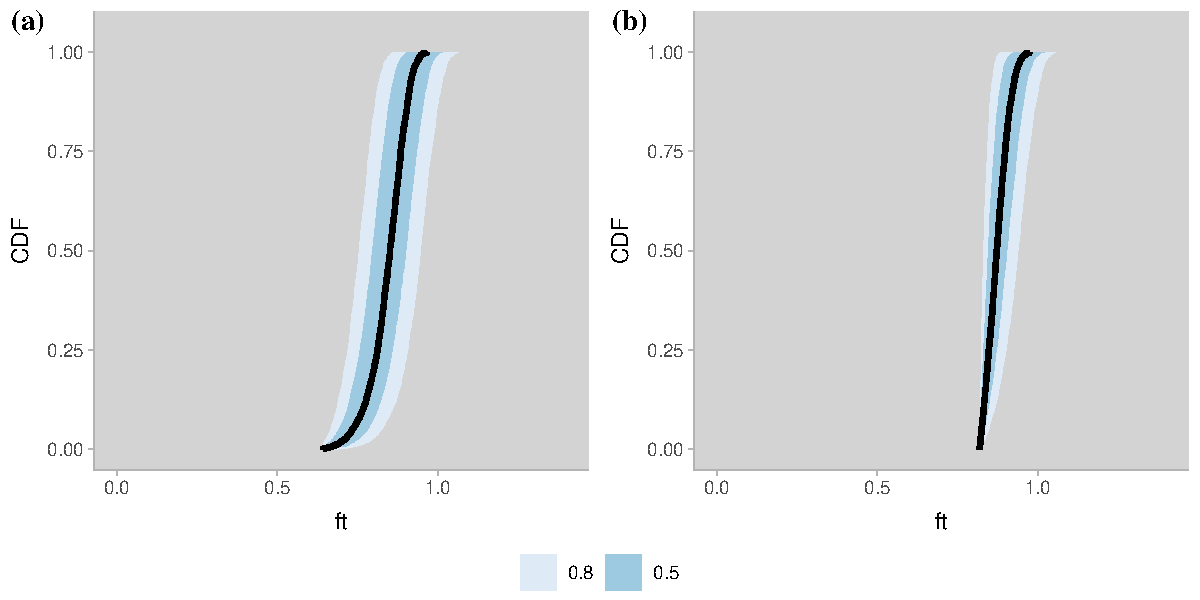
\includegraphics[width=\textwidth]{figures/ch-6/belt_wear_failuretime_CDF_lm.pdf}
  \caption{The failure time CDFs generated from the posterior of the linear general path model conditioned on the first (a) seven and (b) eight observations. The median CDF is indicated by the black line and the uncertainty intervals are shown by the deferent shades of blue ribbons.}
  \label{fig:beltwear-ft-lm}
\end{figure}

\section{Discussions} \label{sec:belt-wear-discussion}

In this chapter, I have constructed, fit, evaluated, and compared two BHMs for conveyor belt wear, and, in doing so, demonstrated an end-to-end example of the Bayesian workflow for an applied problem in the mining industry. In the data models for the two BHMs, I extend FDA to degradation modelling in order to model a degrading surface. In the two process models, I compared the noisy gamma process model from Chaps.~\ref{chap:chapter4} and~\ref{chap:chapter5} with a linear general path model. Lastly, in the parameter models, I show how historical belt wear data can be used to inform the analysis of the current belt through an informative prior. I compare the two models with one another through both visualisations of the posterior draws and the expected log score of N step ahead predictions and also with the method of \cite{webb_2020} in their ability to predict the maximum wear measurement. Lastly, I have shown how to construct failure time distributions based on the current degradation of the belt for the two BHMs. In this last section, I distil the main points of the chapter, discuss the advantages and limitations of the BHM models I have explored and point to areas of future work.

Comparison of the two Bayesian models shows that while both appear to have reasonably fit the data, the linear general path model is a better predictive model for the overall belt's wear based on els. However, when the two models are compared based on their ability to predict the maximum wear observation, which defines the soft failure of the belt, both models' predictions are reasonable when compared with the observed data, and the gamma process model's forecasts are far more optimistic. This optimism is also reflected in the failure time distributions generated from the two models. Consequently, if these models were to be implemented in practice, and using as much of the useful life of the belt as possible was a priority, it would be worthwhile investing in the collection of more detailed data for a short period of time to properly validate the two models, e.g., collecting wear profiles more frequently and measuring more than one location along the belt's length at each time.

An advantage of the BHM structure applied to belt wear is that it can easily incorporate additional observations into the model without the model becoming over-parameterised and can take full advantage of such extra information to reduce the uncertainty of parameter estimates and predictions. This is particularly true for the noisy gamma process model. For example, if we were to have a much finer grid of measurements across the width of the belt's surface at each observation time, these measurements would still be summarised by the same number of spline coefficients. So, the result would be better uncertainty quantification of $\sigma$ with no additional parameters in the lower levels of the hierarchical model. Alternatively, if more than one functional observation was recorded at each observation time, this could be incorporated by drawing more than one realisation of the noisy spline coefficients. To elaborate, instead of a single set of noisy spline coefficients at each time, we could use $y_{j, i, m} \sim N(y^*_{i, m}, y^*_{i, m}\phi)$, where the new subscript $j$ identifies the different functional observation at time $t_i$. The result would be better identification of $\phi$---the spatial variation in wear profiles along the length of the belt---and subsequently a more precise filtered estimate of the $y^*_{i, m}$. Lastly, if observations were collected more frequently, then the finer temporal resolution would better identify the `jumpiness' of the gamma process, i.e., $\nu$ would be estimated more precisely, which in tern refines the uncertainty quantification of the forecasts from the gamma process. 

An alternative extension to these models would be to two-dimensional data. Here, I have shown an application of this model to a one-dimensional surface; however, the method could easily be extended to a two-dimensional wearing surface by using two-dimensional spatial basis functions such as in \citet[p. 84]{wikle_2019}. For the case of belt wear, we could extend the model in this way if there were multiple functional observations at each time, and we knew the location along the length of the belt of each observation. By expanding the model to two dimensions, the method could be applied to the degradation of many other assets---for example, the wear liners in transfer station shoots or haul truck beds.

As I touched on briefly when discussing the prior predictive checks in Section~\ref{sec:belt_wear_priors}, I have made the simplifying assumption that the spline coefficients are independent of one another. In doing so, we neglect any large-scale spatial structure in the wear profiles. For both prior and posterior predictive checks, if we simulate a single belt profile, it will look unrealistically `wiggly'. Although the B-spline accounts for small-scale spatial structure in the UT measurements, the assumed independence of the spline coefficients means that there is no way to capture any large-scale spacial structure. In reality, we would expect neighbouring coefficients to behave somewhat similarly. A possible way of accounting for this large-scale spatial correlation would be to include a spatial random effect, which would most likely result in better uncertainty quantification in the parameter estimates and forecasts since we are adding information about the underlying process through the model's structure. One hurdle to implementing a spatial random effect in the gamma process model is there is no straightforward way of coercing correlation in the jumps of multiple gamma processes. This would be an interesting area for future work. Because of this hurdle, it may be simpler to implement large-scale spatial structure in the linear model. This could be done using a conditional autoregressive structure. Nevertheless, the simplifying assumption of independence appears acceptable since the `wiggliness' of the individual realisations is `washed out' when I average over all of the posterior draws, making any predictions look smooth, such as in Fig.~\ref{fig:beltwear-forecasts}.

When confronted with analysing complicated, small, and messy datasets---something very common in reliability and condition monitoring---a very natural approach is to simplify the data and apply methods we are familiar with, such as regression. However, here I have demonstrated that if we instead take the time to think deeply about how the data arise and what extra knowledge we possess about the data-generating process, we can construct statistical models that take full advantage of all the information available in both the data and our understanding of the problem. In doing so, we get more detailed predictions and defensible uncertainty qualification for the reliability predictions and accompanying maintenance decisions.
\chapter{Discussions}\label{chap:chapter7}

\section{Overview and discussions}

\section{Strengths and limitations}

\section{Future directions}

\section{Implications for industry practitioners}

{
    \backmatter
    \printbibliography
    \noindent
    Every reasonable effort has been made to acknowledge the owners of copyright material.
    I would be pleased to hear from any copyright owner who has been omitted or incorrectly acknowledged.
} % dont have appendix within a backmatter

%%
%% This is a file demonstrating the use of appendix files in the Curtin thesis skeleton
%% file. And can be used as infrastructure to build your thesis.
%%

\chapter{Appendix Title}
\label{app:appendixA}

\end{document}